\chapter{随机变量的数值特征}
\label{chap:random-variable-moments}

掷一枚均匀的骰子：点数是$1$、$2$、$3$时没有奖金，点数是$4$或$5$时得$3$元，点数是$6$时得$6$元。奖金$X$的分布是一张三行的概率表，它回答了每种结果的机会有多大。可是参与之前，人们更想先知道两个数：平均能拿多少钱，以及每次的结果会离这个平均有多远。如果参加一次要付$2.5$元，值不值？另一个游戏平均奖金相同，但输赢更集中，又该怎样比较？

把一整张概率表压缩成少数几个数，会马上遇到三类问题。第一，平均要怎样定义，才能同时处理有限个取值、可数个取值和密度？取值可以无穷多时，加权和可能发散，甚至随求和次序改变。第二，平均满足哪些运算规则，算一个函数的平均时是否必须先求出这个函数的分布？第三，除了平均位置和波动尺度，还有哪些数能描述分布的偏斜与尾部，这些数在什么条件下存在，又能在多大程度上代替分布本身？

本章用上面的奖金表和$(0,1)$上的密度$f_X(x)=2x$作为贯穿全章的两个例子。先定义期望，讲清它的存在条件、运算性质、函数的期望和凸函数的期望；再用期望定义方差，研究计算方法、平移缩放规律和标准化；最后把幂次推广到一般的阶，讨论矩的存在性、计算、偏度与峰度，并说明有限个矩为何不能确定分布。分位数已在第~\ref{chap:random-variables}章定义，这里只在比较均值与中位数时用到它。

\section{期望}
\label{sec:rvm-expectation}

骰子游戏平均能拿多少钱？这个问题要求用一个数概括整张概率表，而且这个数应当按概率给各个取值加权。取值只有有限个时，加权平均就是一个有限和；取值有可数无穷个或由密度给出时，有限和变成级数或积分，就必须先检查它是否有意义。本节先给出定义和存在条件，再建立运算规则，然后说明怎样直接计算函数的平均，最后比较“先平均再变换”与“先变换再平均”。

\subsection{定义}
\label{sec:rvm-expectation-definition}

\paragraph{有限个取值}
设想把骰子游戏玩$6000$次。按概率，大约有$3000$次拿到$0$元，$2000$次拿到$3$元，$1000$次拿到$6$元。总奖金约为
\[
 0\times3000+3\times2000+6\times1000=12000,
\]
平均每次约$2$元。把次数换成比例，这个计算就是按概率加权：
\[
 0\times\tfrac12+3\times\tfrac13+6\times\tfrac16=2 .
\]
重复次数越多，实际平均为什么越接近这个加权和，是第~\ref{chap:laws-of-large-numbers}章大数律的内容。这里只把加权和本身作为定义的出发点，它只用到概率表，与任何一次具体的试验结果无关。

另一种看法来自力学。把总质量$1$按概率分配到数轴上：位置$0$放质量$\tfrac12$，位置$3$放$\tfrac13$，位置$6$放$\tfrac16$。在位置$c$处支起数轴，各质量对支点的力矩之和是$\sum_i(x_i-c)p_X(x_i)$，它等于零时数轴平衡。解出的$c$正是加权和$\sum_ix_ip_X(x_i)=2$。所以加权平均就是这组质量的重心，见图~\ref{fig:rvm-balance}(a)。

\begin{BookInlineFigure}
 \centering
 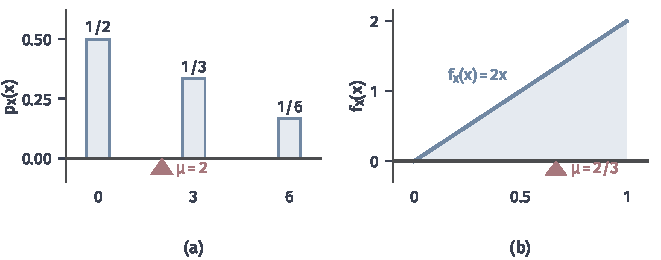
\includegraphics[width=112mm]{figures/07-probability/01-elementary-probability/matplotlib/rvm-balance/figure.pdf}
 \caption{期望是概率质量的重心。(a)奖金表：位置$0,3,6$上分别放质量$\tfrac12,\tfrac13,\tfrac16$（蓝色柱），红色三角是使数轴平衡的支点$\mu=2$，它不是$X$的任何可能取值。(b)密度$f_X(x)=2x$把质量连续地铺在$(0,1)$上，右侧更重，重心在$\mu=2/3$。}
 \label{fig:rvm-balance}
\end{BookInlineFigure}

这个例子说明期望不必是随机变量能取到的值。没有哪一次游戏恰好得$2$元，$2$描述的是质量的平衡位置，而不是某次的典型结果。图中重心偏向左侧，因为一半的质量堆在$0$上；位置$6$虽远，质量却只有$\tfrac16$。

\begin{definition}[有限取值的期望]
\label{def:rvm-expectation-finite}
设随机变量$X$只取有限个值$x_1,\dots,x_n$，概率质量为$p_X(x_i)$。称
\begin{equation}
 \mathbb{E}[X]=\sum_{i=1}^{n}x_i\,p_X(x_i)
 \label{eq:rvm-mean-finite}
\end{equation}
为$X$的\term{期望}（expectation），也称\term{均值}（mean），常记作$\mu$或$\mu_X$。
\end{definition}

\paragraph{从样本点求和}
式~\eqref{eq:rvm-mean-finite}按$X$的取值分组求和。也可以回到试验本身，逐个样本点相加。骰子有六个等可能的点数$\omega=1,\dots,6$，奖金是点数的函数$X(\omega)$。逐点相加得到
\[
 \sum_{\omega=1}^{6}X(\omega)\,\mathbb{P}(\{\omega\})
 =\tfrac16(0+0+0+3+3+6)=2,
\]
与按取值分组的结果相同。图~\ref{fig:rvm-reward-map}显示了这两种算法的关系：先把映到同一个值的样本点归成一组，组内概率之和就是这个值的概率质量。

\begin{BookInlineFigure}
 \centering
 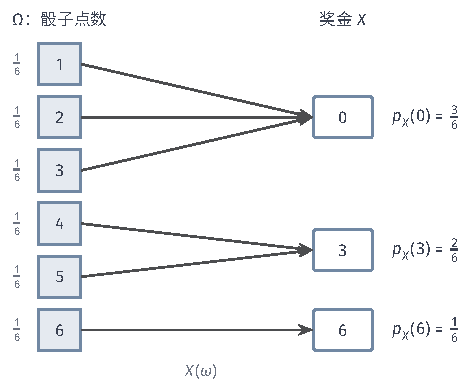
\includegraphics[width=80mm]{figures/07-probability/01-elementary-probability/tikz/rvm-reward-map/figure.pdf}
 \caption{奖金$X$是样本空间$\Omega=\{1,\dots,6\}$上的函数。左侧每个点数的概率是$\tfrac16$；映到同一奖金的点数合成一组，组内概率相加就得到右侧的概率质量。逐点求和与按取值分组求和只是加法的次序不同。}
 \label{fig:rvm-reward-map}
\end{BookInlineFigure}

一般地，若样本空间$\Omega$有限，按$X$的取值把样本点分组，就有
\begin{equation}
 \mathbb{E}[X]=\sum_{\omega\in\Omega}X(\omega)\,\mathbb{P}(\{\omega\}) .
 \label{eq:rvm-mean-sample-points}
\end{equation}
理由是每个样本点恰好落在一组中，而第$i$组的概率之和是$p_X(x_i)$，组内各项的$X(\omega)$都等于$x_i$。有限和可以任意分组与交换次序，所以两种求和结果相同。下一小节将用式~\eqref{eq:rvm-mean-sample-points}证明期望的线性性。

\paragraph{可数个取值}
取值有可数无穷个时，加权和成为级数，这时会出现有限和没有的两个问题：级数可能发散，也可能只在某种求和次序下收敛。先看非负的情形。设$X$取正整数，
\[
 p_X(k)=\frac{1}{k(k+1)},\qquad k=1,2,\dots .
\]
由$\frac{1}{k(k+1)}=\frac1k-\frac1{k+1}$，前$n$项之和是$1-\frac1{n+1}$，它趋于$1$，所以这是一张合法的概率表。

计算加权和时，各项为$k\,p_X(k)=\frac{1}{k+1}$，于是部分和
\[
 \sum_{k=1}^{n}k\,p_X(k)=\sum_{k=1}^{n}\frac{1}{k+1}
\]
随$n$无限增大，增长速度与$\ln n$相同，见图~\ref{fig:rvm-truncated-sums}(a)。各项都非负，部分和单调增加，所以无论按什么次序相加，结果都是$+\infty$。对非负随机变量，这样的结论有明确含义：平均没有上限，我们写$\mathbb{E}[X]=+\infty$。用重心的语言说，质量$\frac{1}{k(k+1)}$随距离$k$衰减得不够快，远处的质量对力矩的贡献加起来没有上界，数轴在任何位置都无法平衡。

有正有负的取值则不同。若正负两部分的加权和都是$+\infty$，部分和的极限取决于正项与负项轮流加入的方式。由级数重排定理，条件收敛的级数重排后可以收敛到任意指定的值，可参考\BookChapterRef{chap:limits-continuity}{卷一第5章“极限与连续”}。概率表里的取值并没有天然的先后次序，所以只有与次序无关的和才适合作为期望。解决办法是把正负两部分分开计算。

\paragraph{正部与负部}
对实数$x$，记$x^{+}=\max\{x,0\}$，$x^{-}=\max\{-x,0\}$，则
\begin{equation}
 x=x^{+}-x^{-},\qquad \lvert x\rvert=x^{+}+x^{-} .
 \label{eq:rvm-pos-neg}
\end{equation}
对随机变量逐个取值使用这两个函数，得到两个非负随机变量$X^{+}$与$X^{-}$，分别称为$X$的\term{正部}（positive part）与\term{负部}（negative part）。$X^{+}$只记录收益，$X^{-}$只记录损失，两者都非负，它们的加权和总有意义，可能是有限数，也可能是$+\infty$。

\paragraph{密度的情形}
有密度时，概率质量连续地铺在数轴上，单位长度上的质量是$f_X(x)$。把小区间$[x,x+\mathrm{d}x]$上的质量$f_X(x)\,\mathrm{d}x$看作放在$x$处，加权和就变成积分。对贯穿例子$f_X(x)=2x$（$0<x<1$），有
\[
 \int_0^1x\cdot2x\,\mathrm{d}x=\left[\tfrac23x^{3}\right]_0^1=\tfrac23 .
\]
图~\ref{fig:rvm-balance}(b)中质量向右堆积，重心落在$2/3$，比区间中点$1/2$偏右。

密度的支撑无界时，积分是反常积分，同样要分正负两部分检查。考虑对称的密度
\[
 f_X(x)=\frac{1}{2x^{2}},\qquad \lvert x\rvert\geq1 .
\]
它在$[1,\infty)$与$(-\infty,-1]$上各有质量$\tfrac12$，总质量为一。正部的积分是
\[
 \int_1^{\infty}x\cdot\frac{1}{2x^{2}}\,\mathrm{d}x=\frac12\int_1^{\infty}\frac{\mathrm{d}x}{x}=+\infty,
\]
负部同理也是$+\infty$。

两侧都无穷时，截断的方式决定了截断后的积分。在$[-a,b]$（$a,b\geq1$）上，正负两侧的贡献分别是$\frac12\ln b$与$-\frac12\ln a$，所以截断积分为$\frac12\ln(b/a)$。对称截断$b=a$得$0$，截断$b=2a$恒得$\frac12\ln2\approx0.35$，截断$b=a^{2}$得$\frac12\ln a\to+\infty$。图~\ref{fig:rvm-truncated-sums}(b)画出了这三种截断。密度关于$0$对称，却不能因此说期望是$0$：期望根本没有定义。

\begin{BookInlineFigure}
 \centering
 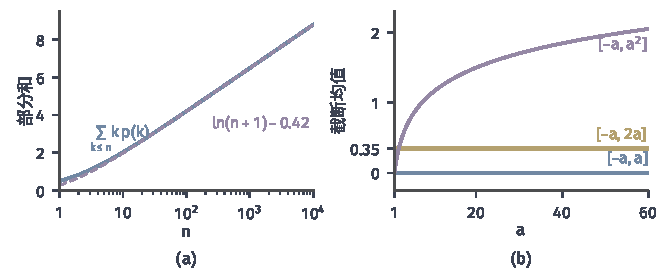
\includegraphics[width=112mm]{figures/07-probability/01-elementary-probability/matplotlib/rvm-truncated-sums/figure.pdf}
 \caption{无穷的加权和。(a)概率表$p_X(k)=1/[k(k+1)]$的部分和$\sum_{k\leq n}k\,p_X(k)$（蓝）与$\ln(n+1)-0.42$（紫色虚线）几乎重合，趋于$+\infty$。(b)对称密度$1/(2x^{2})$（$\lvert x\rvert\geq1$）在$[-a,b]$上的截断积分$\frac12\ln(b/a)$：对称截断（蓝）恒为$0$，$b=2a$（黄）恒为$0.35$，$b=a^{2}$（紫）无界增长。}
 \label{fig:rvm-truncated-sums}
\end{BookInlineFigure}

\paragraph{期望的定义}
上面的例子给出了三种情形：非负变量的加权和总有意义，可能为$+\infty$；有正有负时，只要正负两部分不同时为无穷，差仍有意义；两部分都无穷时没有合理的值。下面的定义同时覆盖概率表与密度。

\begin{definition}[期望]
\label{def:rvm-expectation}
设$X$是取有限或可数个值$x_i$的离散随机变量，概率质量为$p_X$；或$X$有密度$f_X$。$X$的正部与负部的期望定义为
\begin{equation}
 \begin{aligned}
 \mathbb{E}[X^{+}]&=\sum_{x_i>0}x_i\,p_X(x_i)\quad\text{或}\quad\int_0^{\infty}x\,f_X(x)\,\mathrm{d}x,\\
 \mathbb{E}[X^{-}]&=\sum_{x_i<0}(-x_i)\,p_X(x_i)\quad\text{或}\quad\int_{-\infty}^{0}(-x)\,f_X(x)\,\mathrm{d}x,
 \end{aligned}
 \label{eq:rvm-mean-parts}
\end{equation}
它们取值于$[0,+\infty]$。若两者不同时为$+\infty$，定义
\begin{equation}
 \mathbb{E}[X]=\mathbb{E}[X^{+}]-\mathbb{E}[X^{-}] .
 \label{eq:rvm-mean-general}
\end{equation}
若两者都有限，等价地
\begin{equation}
 \mathbb{E}\lvert X\rvert=\mathbb{E}[X^{+}]+\mathbb{E}[X^{-}]<\infty,
 \label{eq:rvm-integrable}
\end{equation}
称$X$\term{可积}（integrable），这时期望是有限实数，并且
\begin{equation}
 \mathbb{E}[X]=\sum_{i}x_i\,p_X(x_i)\quad\text{或}\quad\mathbb{E}[X]=\int_{-\infty}^{\infty}x\,f_X(x)\,\mathrm{d}x,
 \label{eq:rvm-mean-sum-integral}
\end{equation}
其中级数按任何次序求和都绝对收敛，积分是绝对收敛的反常积分。
\end{definition}

定义中三层条件各起不同作用。非负变量的期望总存在，只是可能为$+\infty$，例如$p_X(k)=1/[k(k+1)]$的$X$。有符号变量需要检查正负两部分，只有一侧无穷时期望是$+\infty$或$-\infty$，两侧都无穷时期望不存在，例如上面的对称密度。说“期望有限”或“$X$可积”都要求$\mathbb{E}\lvert X\rvert<\infty$，绝对收敛保证了式~\eqref{eq:rvm-mean-sum-integral}与求和次序、截断方式都无关。

只取有限个值的变量总是可积的，定义~\ref{def:rvm-expectation}在这时就回到式~\eqref{eq:rvm-mean-finite}。取值有界的变量也总是可积：若$\lvert X\rvert\leq M$，则$\mathbb{E}\lvert X\rvert\leq M$。期望可能不存在的情形都来自远处的质量，第~\ref{chap:common-distributions}章会在具体的分布中再次遇到这种现象。

\paragraph{兼有点质量与密度的模型}
有的模型同时含有点质量和连续部分，例如等待时间以概率$0.3$恰为$0$，其余概率$0.7$按密度$0.7\,\mathrm{e}^{-t}$（$t>0$）分布。这时把两部分的贡献相加，
\[
 \mathbb{E}[T]=0\times0.3+\int_0^{\infty}t\cdot0.7\,\mathrm{e}^{-t}\,\mathrm{d}t=0.7 .
\]
这种加法与定义~\ref{def:rvm-expectation}的精神一致，但概率表和密度都不能单独描述这类分布。对一般分布统一的期望定义要借助概率空间上的积分，在第~\ref{chap:probability-spaces}章完成。本部分只用离散求和、密度积分以及两者之和。

\subsection{基本性质}
\label{sec:rvm-expectation-properties}

两个游戏的奖金之和平均是多少？如果期望能逐项相加，只需分别知道两个平均；若不能，就得先求和的完整分布。下面的性质说明，在可积条件下期望对线性组合可以逐项计算，而且不需要任何独立性假设。

\paragraph{线性性、保序性与绝对值估计}
为了让多个随机变量同时有意义，设它们定义在同一个样本空间$\Omega$上。这里先在$\Omega$有限或可数、每个样本点有概率$\mathbb{P}(\{\omega\})$的情形证明，此时期望可以像式~\eqref{eq:rvm-mean-sample-points}那样逐点求和。对可数的$\Omega$，$X$可积等价于$\sum_{\omega}\lvert X(\omega)\rvert\,\mathbb{P}(\{\omega\})<\infty$，按取值分组的论证与有限情形相同，只是用到了绝对收敛级数可以任意分组。

\begin{theorem}[期望的基本性质]
\label{thm:rvm-expectation-properties}
设$X,Y$是同一样本空间上的可积随机变量，$a,b,c$为实数。
(1)线性性：$aX+bY+c$可积，且
\begin{equation}
 \mathbb{E}[aX+bY+c]=a\,\mathbb{E}[X]+b\,\mathbb{E}[Y]+c .
 \label{eq:rvm-linearity}
\end{equation}
(2)保序性：若对每个样本点$X(\omega)\leq Y(\omega)$，则$\mathbb{E}[X]\leq\mathbb{E}[Y]$。
(3)绝对值估计：
\begin{equation}
 \lvert\mathbb{E}[X]\rvert\leq\mathbb{E}\lvert X\rvert .
 \label{eq:rvm-abs-bound}
\end{equation}
\end{theorem}

\begin{proof}
在$\Omega$有限或可数时证明。记$q(\omega)=\mathbb{P}(\{\omega\})$。

线性性。由三角不等式，对每个$\omega$有
\[
 \lvert aX(\omega)+bY(\omega)+c\rvert\leq\lvert a\rvert\,\lvert X(\omega)\rvert+\lvert b\rvert\,\lvert Y(\omega)\rvert+\lvert c\rvert .
\]
两边乘$q(\omega)$后求和，右边是$\lvert a\rvert\,\mathbb{E}\lvert X\rvert+\lvert b\rvert\,\mathbb{E}\lvert Y\rvert+\lvert c\rvert<\infty$，所以$aX+bY+c$可积。三个绝对收敛级数可以逐项相加，于是
\[
 \begin{aligned}
 &\sum_{\omega}\bigl(aX(\omega)+bY(\omega)+c\bigr)q(\omega)\\
 &\quad=a\sum_{\omega}X(\omega)q(\omega)+b\sum_{\omega}Y(\omega)q(\omega)+c\sum_{\omega}q(\omega),
 \end{aligned}
\]
最后一个和等于$1$，这就是式~\eqref{eq:rvm-linearity}。

保序性。$Y-X$在每个样本点非负，所以$\sum_{\omega}(Y(\omega)-X(\omega))q(\omega)\geq0$。由线性性，左边等于$\mathbb{E}[Y]-\mathbb{E}[X]$。

绝对值估计。逐点有$-\lvert X\rvert\leq X\leq\lvert X\rvert$，由保序性得
\[
 -\mathbb{E}\lvert X\rvert\leq\mathbb{E}[X]\leq\mathbb{E}\lvert X\rvert .
\]
\end{proof}

线性性的证明只用到求和的线性，没有涉及$X$与$Y$之间的任何关系。这一点非常有用：一个复杂的计数常常可以拆成许多简单的指示变量，各自求平均再相加，而不必弄清它们怎样相互影响。对有密度的变量，$aX+b$的情形在下一小节由函数的期望直接得到；两个不同变量之和$X+Y$的期望需要它们的联合分布，在第~\ref{chap:random-vectors}章证明，一般的随机变量在第~\ref{chap:probability-spaces}章统一处理。三条性质在这些情形中都保持不变。

保序性有一个常用的推论。若$a\leq X\leq b$，把常数看作随机变量，就得到$a\leq\mathbb{E}[X]\leq b$。对奖金表，$0\leq X\leq6$，所以期望必须落在$[0,6]$中，$2$确实在其中。

\paragraph{线性性不需要独立}
把编号为$1,2,3$的三封信随机装进编号为$1,2,3$的三个信封，六种装法等可能。平均有几封信装对了信封？设$N$是装对的封数，$I_j$在第$j$封信装对时取$1$、否则取$0$，则
\[
 N=I_1+I_2+I_3 .
\]
$I_j$只取$0$和$1$，它的期望是$1\cdot\mathbb{P}(I_j=1)+0\cdot\mathbb{P}(I_j=0)$，即取$1$的概率。第$j$封信落在每个信封的机会相同，所以
\[
 \mathbb{E}[I_j]=\mathbb{P}(\text{第}j\text{封装对})=\tfrac13 .
\]
由线性性，
\[
 \mathbb{E}[N]=\tfrac13+\tfrac13+\tfrac13=1 .
\]

这三个指示变量并不独立。由图~\ref{fig:rvm-fixed-points}，前两封都装对只有一种装法，概率为$\tfrac16$，而不是$\tfrac13\times\tfrac13=\tfrac19$；前两封装对时第三封必然也装对。直接从表中计算，$N$取$3,1,1,0,0,1$，平均也是$\tfrac16(3+1+1+0+0+1)=1$，与线性性的结果一致。信封数换成$n$时，同样的论证给出$\mathbb{E}[N]=n\cdot\tfrac1n=1$，而$N$的完整分布要用容斥原理才能求出。

\begin{BookInlineFigure}
 \centering
 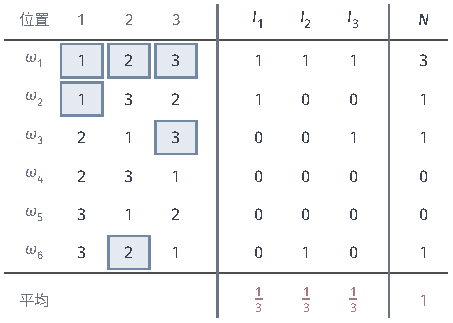
\includegraphics[width=77mm]{figures/07-probability/01-elementary-probability/tikz/rvm-fixed-points/figure.pdf}
 \caption{三封信装入三个信封的六种等可能方式。每行列出各位置装入的信，蓝框表示装对。$I_j$记录第$j$封是否装对，$N=I_1+I_2+I_3$。各列平均（红）满足$\tfrac13+\tfrac13+\tfrac13=1$，尽管$I_1,I_2,I_3$相互依赖。}
 \label{fig:rvm-fixed-points}
\end{BookInlineFigure}

\paragraph{乘积与无穷和}
线性性只涉及加法和数乘。乘积的期望一般不能拆开：取$Y=X$为奖金，则
\[
 \mathbb{E}[XY]=\mathbb{E}[X^{2}]=0\times\tfrac12+9\times\tfrac13+36\times\tfrac16=9,
\]
而$\mathbb{E}[X]\,\mathbb{E}[Y]=4$。乘积可以拆开的充分条件是独立，这需要联合分布，在第~\ref{chap:random-vectors}章讨论。

线性性对有限个变量成立。对无穷多个变量之和，等式
\[
 \mathbb{E}\Bigl[\sum_{k=1}^{\infty}X_k\Bigr]=\sum_{k=1}^{\infty}\mathbb{E}[X_k]
\]
相当于交换求和与取极限的次序，需要非负性或绝对可和这样的额外条件。这类交换的一般依据在第~\ref{chap:probability-spaces}章由积分的收敛定理给出。

\subsection{函数的期望}
\label{sec:rvm-function-expectation}

奖金的平方平均是多少？按定义，应当先求出新变量$Y=X^{2}$的概率表：$Y$取$0,9,36$，概率依次为$\tfrac12,\tfrac13,\tfrac16$，再加权得$9$。上一小节正是这样做的。但这个结果也可以不写出$Y$的分布，直接在$X$的每个取值上计算$x^{2}$再加权。下面的定理说明这种直接计算总是正确的，只要相应的和或积分绝对收敛。

\begin{theorem}[函数的期望]
\label{thm:rvm-lotus}
设$g$是实值函数。
\begin{enumerate}
 \item 若$X$离散，取值$x_i$，且$\sum_i\lvert g(x_i)\rvert\,p_X(x_i)<\infty$，则$g(X)$可积，且
 \begin{equation}
  \mathbb{E}[g(X)]=\sum_{i}g(x_i)\,p_X(x_i) .
  \label{eq:rvm-lotus-discrete}
 \end{equation}
 \item 若$X$有密度$f_X$，$g$分段连续，且$\int_{-\infty}^{\infty}\lvert g(x)\rvert f_X(x)\,\mathrm{d}x<\infty$，则$g(X)$可积，且
 \begin{equation}
  \mathbb{E}[g(X)]=\int_{-\infty}^{\infty}g(x)\,f_X(x)\,\mathrm{d}x .
  \label{eq:rvm-lotus-density}
 \end{equation}
\end{enumerate}
若$g\geq0$，两式在不要求有限的情况下也成立，两边同时为有限数或同时为$+\infty$。
\end{theorem}

\begin{proof}
离散情形。$Y=g(X)$的取值是集合$\{g(x_i)\}$中的数。对每个$y$，事件$\{Y=y\}$是若干个事件$\{X=x_i\}$（$g(x_i)=y$）的并，所以
\[
 p_Y(y)=\sum_{i:\,g(x_i)=y}p_X(x_i) .
\]
代入$Y$的期望，再把对$y$与对$i$的二重和合并成对$i$的一重和，得到
\[
 \sum_{y}y\,p_Y(y)=\sum_{y}\sum_{i:\,g(x_i)=y}g(x_i)\,p_X(x_i)=\sum_{i}g(x_i)\,p_X(x_i) .
\]
最后一步中每个$i$恰好出现在$y=g(x_i)$那一组。对$\lvert g\rvert$作同样的计算，得到
\[
 \mathbb{E}\lvert Y\rvert=\sum_i\lvert g(x_i)\rvert\,p_X(x_i)<\infty,
\]
所以$Y$可积，而绝对收敛保证了上面的重新分组不改变和。$g\geq0$时各项非负，重新分组同样不改变和，结论对$+\infty$也成立。

密度情形只证$g$在$X$的取值区间$(\alpha,\beta)$上连续可微且$g'>0$的情形。这时$g$把$(\alpha,\beta)$一一映成区间$(g(\alpha^{+}),g(\beta^{-}))$，记反函数为$h$。由$\{g(X)\leq y\}=\{X\leq h(y)\}$，
\[
 F_Y(y)=F_X\bigl(h(y)\bigr),\qquad f_Y(y)=f_X\bigl(h(y)\bigr)\,h'(y) .
\]
先设$g\geq0$。在$\int y\,f_Y(y)\,\mathrm{d}y$中作换元$y=g(x)$，$h(y)=x$，$\mathrm{d}y=g'(x)\,\mathrm{d}x$，并利用$h'(g(x))g'(x)=1$，得到
\[
 \int y\,f_X\bigl(h(y)\bigr)h'(y)\,\mathrm{d}y=\int_{\alpha}^{\beta}g(x)\,f_X(x)\,\mathrm{d}x .
\]
被积函数非负，反常积分的换元对有限值和$+\infty$都成立。一般的$g$对正部$g^{+}$与负部$g^{-}$分别使用这一结论再相减。$g'<0$时换元会交换积分上下限，结论相同。
\end{proof}

密度情形的一般证明需要先求出$g(X)$的分布，而$g(X)$可能根本没有密度，例如$g$是指示函数或在某个区间上为常数。第~\ref{chap:random-variable-transformations}章用换元公式处理分段单调的$g$，第~\ref{chap:probability-spaces}章把式~\eqref{eq:rvm-lotus-density}作为推前分布上的积分一般地证明。在这之前，我们在定理的条件下使用它。

定理中的绝对可积条件要对每个$g$分别检查，它与$X$本身是否可积无关。例如密度$f_X(x)=x^{-2}$（$x\geq1$）的$X$满足
\[
 \mathbb{E}[X]=\int_1^{\infty}x\cdot x^{-2}\,\mathrm{d}x=+\infty,
\]
但
\[
 \mathbb{E}\bigl[\sqrt{X}\bigr]=\int_1^{\infty}x^{1/2}\cdot x^{-2}\,\mathrm{d}x=\int_1^{\infty}x^{-3/2}\,\mathrm{d}x=2,
\]
增长较慢的函数仍可积。反过来，$X$可积也不保证$X^{2}$可积，第~\ref{sec:rvm-moments}节会系统地讨论这一点。

\paragraph{指示函数：概率也是期望}
取$g=\mathbf{1}_{A}$，它在$x\in A$时为$1$，否则为$0$。式~\eqref{eq:rvm-lotus-discrete}或式~\eqref{eq:rvm-lotus-density}的右边只剩下$A$上的质量，于是
\begin{equation}
 \mathbb{E}\bigl[\mathbf{1}_{A}(X)\bigr]=\mathbb{P}(X\in A) .
 \label{eq:rvm-indicator}
\end{equation}
概率因此是期望的特殊情形，信封例子中$\mathbb{E}[I_j]=\tfrac13$用的正是这一点。对奖金表取$A=(0,\infty)$，得到中奖的概率$\tfrac13+\tfrac16=\tfrac12$。

\paragraph{收益：不必先求新变量的分布}
奖金本身就是点数的函数。设$D$是骰子点数，$g(1)=g(2)=g(3)=0$，$g(4)=g(5)=3$，$g(6)=6$，则$X=g(D)$。由式~\eqref{eq:rvm-lotus-discrete}，
\[
 \mathbb{E}[g(D)]=\tfrac16\bigl(g(1)+\dots+g(6)\bigr)=\tfrac16(0+0+0+3+3+6)=2,
\]
与先求$X$的概率表再加权的结果相同。若参加一次要付$2.5$元，净收益是$g(D)-2.5$，由线性性它的期望是$-0.5$元，长期参加平均每次亏$0.5$元。

连续的例子也一样。设$X$的密度是$2x$（$0<x<1$），$Y=X^{2}$。直接计算
\[
 \mathbb{E}[X^{2}]=\int_0^1x^{2}\cdot2x\,\mathrm{d}x=\tfrac12 .
\]
另一方面，对$0<y<1$有
\[
 F_Y(y)=\mathbb{P}(X\leq\sqrt{y})=\int_0^{\sqrt{y}}2x\,\mathrm{d}x=y,
\]
所以$Y$在$(0,1)$上有常数密度$1$，$\mathbb{E}[Y]=\int_0^1y\,\mathrm{d}y=\tfrac12$。两条途径对应图~\ref{fig:rvm-square-transform}中两块面积，它们相等。

\begin{BookInlineFigure}
 \centering
 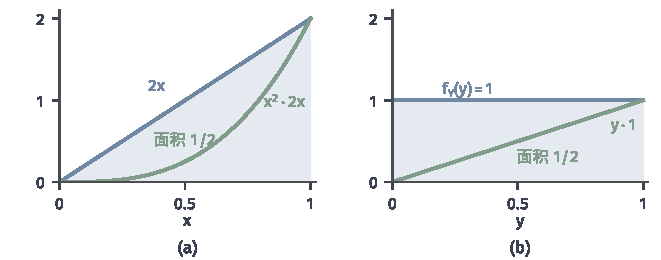
\includegraphics[width=112mm]{figures/07-probability/01-elementary-probability/matplotlib/rvm-square-transform/figure.pdf}
 \caption{用两种方式计算$\mathbb{E}[X^{2}]$，$X$的密度为$2x$。(a)在$X$的尺度上积分$x^{2}\cdot2x$（绿色曲线下的面积）；(b)先求出$Y=X^{2}$的密度$f_Y(y)=1$，再积分$y\cdot1$（绿色直线下的面积）。两块面积都是$1/2$。}
 \label{fig:rvm-square-transform}
\end{BookInlineFigure}

\paragraph{平方误差与绝对误差}
如果要用一个常数$c$预测奖金，平方误差的平均是多少？设$\mathbb{E}[X^{2}]<\infty$，记$\mu=\mathbb{E}[X]$。把$X-c$写成$(X-\mu)+(\mu-c)$后展开，由线性性，交叉项的期望是$2(\mu-c)\,\mathbb{E}[X-\mu]=0$，于是
\begin{equation}
 \mathbb{E}\bigl[(X-c)^{2}\bigr]=\mathbb{E}\bigl[(X-\mu)^{2}\bigr]+(\mu-c)^{2} .
 \label{eq:rvm-square-error}
\end{equation}
右边第二项只在$c=\mu$时为零，所以期望是平方误差意义下最好的常数预测。对奖金表，偏差$X-2$取$-2,1,4$，
\[
 \mathbb{E}\bigl[(X-2)^{2}\bigr]=4\cdot\tfrac12+1\cdot\tfrac13+16\cdot\tfrac16=5,
\]
因此
\[
 \mathbb{E}\bigl[(X-c)^{2}\bigr]=5+(c-2)^{2},
\]
它是图~\ref{fig:rvm-error-curves}(a)中的抛物线，最低点为$(2,5)$。最小值$5$是下一节的方差。

把平方换成绝对值，结论就变了。对奖金表，
\[
 \mathbb{E}\lvert X-c\rvert=\tfrac12\lvert c\rvert+\tfrac13\lvert3-c\rvert+\tfrac16\lvert6-c\rvert .
\]
逐段去掉绝对值：$c<0$时它等于$2-c$，$0\leq c\leq3$时等于常数$2$，$3\leq c\leq6$时等于$\tfrac23c$，$c>6$时等于$c-2$。最小值在整个区间$[0,3]$上取到。这个区间正是使$\mathbb{P}(X\leq c)\geq\tfrac12$且$\mathbb{P}(X\geq c)\geq\tfrac12$的点，即奖金的全部中位数。

\begin{BookInlineFigure}
 \centering
 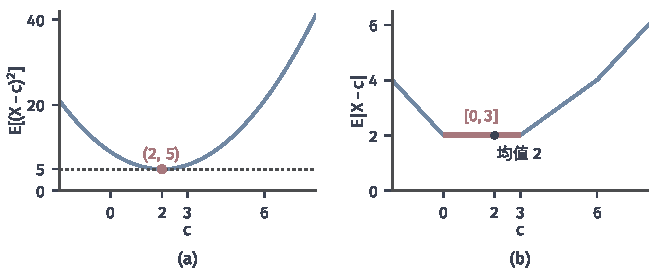
\includegraphics[width=112mm]{figures/07-probability/01-elementary-probability/matplotlib/rvm-error-curves/figure.pdf}
 \caption{用常数$c$预测奖金$X$的平均误差。(a)平方误差$\mathbb{E}[(X-c)^{2}]=5+(c-2)^{2}$在均值$c=2$处取最小值$5$（红点）。(b)绝对误差$\mathbb{E}\lvert X-c\rvert$是折线，在中位数构成的区间$[0,3]$（红色粗线）上取最小值$2$，均值$2$（黑点）恰好也在其中。}
 \label{fig:rvm-error-curves}
\end{BookInlineFigure}

图~\ref{fig:rvm-error-curves}(b)的斜率解释了原因：当$c$不是取值点时，$c$右移一个单位，左侧质量$\mathbb{P}(X<c)$的误差各增加一，右侧质量$\mathbb{P}(X>c)$的误差各减少一，斜率是$\mathbb{P}(X<c)-\mathbb{P}(X>c)$。左右质量相等时斜率为零，这就是中位数的条件。均值与中位数因此回答不同的问题：均值使平方误差最小，受远处取值的影响大；中位数使绝对误差最小，只看质量在左右两侧的分配。若把奖金$6$换成$60$，均值从$2$变成$11$，中位数区间仍是$[0,3]$。

\subsection{凸函数的期望}
\label{sec:rvm-convex-expectation}

先平均再平方，与先平方再平均，结果一样吗？对奖金表，$(\mathbb{E}[X])^{2}=4$，而$\mathbb{E}[X^{2}]=9$。一般地，对非线性函数$f$，$\mathbb{E}[f(X)]$与$f(\mathbb{E}[X])$不相等，但对凸函数两者总有确定的大小关系。这个关系在后面比较风险、比较信息量时反复使用。

\paragraph{有限加权平均}
回忆凸函数的定义：区间$I$上的$f$对一切$x,y\in I$与$\lambda\in[0,1]$满足
\[
 f\bigl(\lambda x+(1-\lambda)y\bigr)\leq\lambda f(x)+(1-\lambda)f(y),
\]
即两点间的图像不高于弦，可参考\BookChapterRef{chap:univariate-differentiation}{卷一第6章“一元函数的微分”}。两点的情形推广到有限个点，就得到下面的引理。

\begin{lemma}[有限加权平均的凸性]
\label{lem:rvm-jensen-finite}
设$f$是区间$I$上的凸函数，点$x_1,\dots,x_n$都在$I$中，权重$\lambda_1,\dots,\lambda_n$非负且和为一。则
\begin{equation}
 f\Bigl(\sum_{i=1}^{n}\lambda_ix_i\Bigr)\leq\sum_{i=1}^{n}\lambda_if(x_i) .
 \label{eq:rvm-jensen-finite}
\end{equation}
\end{lemma}

\begin{proof}
对$n$归纳。$n=1$时两边相等，$n=2$时就是凸函数的定义。设结论对$n-1$个点成立。若$\lambda_n=1$，其余权重都为零，结论成立。否则记$s=1-\lambda_n>0$，令
\[
 \bar{x}=\sum_{i=1}^{n-1}\frac{\lambda_i}{s}x_i .
\]
权重$\lambda_i/s$非负且和为一，$\bar{x}$是$I$中点的加权平均，仍在区间$I$中，并且$\sum_{i}\lambda_ix_i=s\bar{x}+\lambda_nx_n$。先用两点的凸性，再对$\bar{x}$用归纳假设，得到
\[
 f\bigl(s\bar{x}+\lambda_nx_n\bigr)\leq sf(\bar{x})+\lambda_nf(x_n)\leq s\sum_{i=1}^{n-1}\frac{\lambda_i}{s}f(x_i)+\lambda_nf(x_n),
\]
右边等于$\sum_{i=1}^{n}\lambda_if(x_i)$。
\end{proof}

引理有一个直观的重心解释。把质量$\lambda_i$放在图像上的点$(x_i,f(x_i))$，这组质量的重心是$\bigl(\sum\lambda_ix_i,\sum\lambda_if(x_i)\bigr)$，它落在这些点的凸包内。凸函数的图像向下弯，凸包整个位于图像上方或图像上，所以重心的高度不低于图像在同一横坐标处的高度。图~\ref{fig:rvm-jensen}(a)用奖金表画出了这一点：三个点$(0,0)$、$(3,9)$、$(6,36)$的重心是$(2,9)$，图像在$x=2$处的高度只有$4$。

\paragraph{支撑线}
推广到可数个取值和密度时，不能再逐点归纳，需要另一个工具：在凸函数图像上任一内点处，总可以放一条不高于图像的直线。

\begin{lemma}[凸函数的支撑线]
\label{lem:rvm-support-line}
设$f$是开区间$I$上的凸函数，$m\in I$。存在实数$s$，使对一切$x\in I$，
\begin{equation}
 f(x)\geq f(m)+s(x-m) .
 \label{eq:rvm-support-line}
\end{equation}
若$f$在$m$处可微，可取$s=f'(m)$。若$f$严格凸，则$x\neq m$时不等式严格成立。
\end{lemma}

\begin{proof}
取$x<m<y$，均在$I$中。把$m$写成$x$与$y$的凸组合，由凸性得到弦的斜率关系
\[
 \frac{f(m)-f(x)}{m-x}\leq\frac{f(y)-f(m)}{y-m},
\]
这正是上面所引可微凸函数刻画的证明第一步，那一步没有用到可微性。上式对一切$x<m$与$y>m$成立，所以左边对$x$的上确界$L$不超过右边对$y$的下确界$R$，两者都是有限数。取$s\in[L,R]$。对$x<m$，由$\frac{f(m)-f(x)}{m-x}\leq s$得$f(x)\geq f(m)+s(x-m)$；对$y>m$，由$\frac{f(y)-f(m)}{y-m}\geq s$得同一不等式。可微时左右两侧的斜率都趋于$f'(m)$，所以$L=R=f'(m)$。

若$f$严格凸，假设某个$x\neq m$使等号成立，不妨设$x>m$。$f$在$x$与$m$处都与直线$\ell(t)=f(m)+s(t-m)$相等，取中点$z=(x+m)/2$，严格凸性给出$f(z)<\frac12f(m)+\frac12f(x)=\ell(z)$，与$f\geq\ell$矛盾。
\end{proof}

\paragraph{Jensen不等式}
有了支撑线，在$m=\mathbb{E}[X]$处放一条支撑线再取期望，就得到对一般随机变量成立的不等式。

\begin{theorem}[Jensen不等式]
\label{thm:rvm-jensen}
设$f$是开区间$I$上的凸函数，$X$的取值都在$I$中，$X$与$f(X)$都可积。则$\mathbb{E}[X]\in I$，且
\begin{equation}
 f\bigl(\mathbb{E}[X]\bigr)\leq\mathbb{E}\bigl[f(X)\bigr] .
 \label{eq:rvm-jensen}
\end{equation}
若$f$严格凸，等号成立当且仅当$X$以概率一等于常数$\mathbb{E}[X]$。
\end{theorem}

\begin{proof}
先说明$m=\mathbb{E}[X]$在$I$中。设$I$的左端点$\alpha$有限，$X-\alpha$的取值都为正。离散时，$\mathbb{E}[X]-\alpha=\sum_i(x_i-\alpha)p_X(x_i)$中各项非负且总有正项；有密度时，被积函数$(x-\alpha)f_X(x)$非负，且$X$落在某个$[\alpha+\delta,\infty)$中的概率为正，于是积分至少是$\delta$乘这个概率。两种情形都有$m>\alpha$。右端点同理，所以$m\in I$。

由引理~\ref{lem:rvm-support-line}，存在$s$使$f(x)\geq f(m)+s(x-m)$对一切$x\in I$成立。把$x$换成$X$，两边都是可积的随机变量，由保序性与线性性，
\[
 \mathbb{E}[f(X)]\geq f(m)+s\bigl(\mathbb{E}[X]-m\bigr)=f(m) .
\]

等号情形。记$D(x)=f(x)-f(m)-s(x-m)\geq0$，则$\mathbb{E}[D(X)]=\mathbb{E}[f(X)]-f(m)$。$f$严格凸时，$x\neq m$有$D(x)>0$。若$X$离散且$\mathbb{P}(X\neq m)>0$，和式$\sum_iD(x_i)\,p_X(x_i)$中有正项，所以$\mathbb{E}[D(X)]>0$。若$X$有密度，单点$m$的概率为零，总可以找到一个不含$m$的闭区间，使$X$落在其中的概率为正；凸函数在开区间上连续，$D$在这个闭区间上有正的最小值，于是$\mathbb{E}[D(X)]>0$。反过来，$X$以概率一等于$m$时$f(X)$以概率一等于$f(m)$，两边相等。
\end{proof}

定理的条件各有用处。区间取开区间，是为了让$m$成为内点，从而支撑线存在；在闭区间的端点处，凸函数可能没有有限斜率的支撑线，例如$-\sqrt{x}$在$0$处。$X$与$f(X)$可积，保证了取期望时两边都是有限数并可以用线性性。若$f(X)$只是非负而期望为$+\infty$，不等式按$+\infty$理解仍然成立。

\begin{BookInlineFigure}
 \centering
 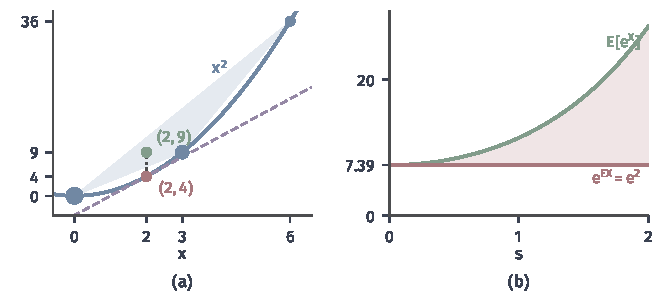
\includegraphics[width=112mm]{figures/07-probability/01-elementary-probability/matplotlib/rvm-jensen/figure.pdf}
 \caption{Jensen不等式的几何。(a)$f(x)=x^{2}$与奖金表：蓝点$(x_i,x_i^{2})$按概率大小画出，浅蓝三角是它们的凸包，重心$(\mathbb{E}[X],\mathbb{E}[X^{2}])=(2,9)$（绿）高于$(2,f(2))=(2,4)$（红）；紫色虚线是$x=2$处的支撑线$y=4+4(x-2)$。(b)$X$以各$\tfrac12$的概率取$2\pm s$时，$\mathbb{E}[\mathrm{e}^{X}]=\mathrm{e}^{2}\cosh s$（绿）与$\mathrm{e}^{\mathbb{E}[X]}=\mathrm{e}^{2}$（红）之差（浅红）随$s$增大。}
 \label{fig:rvm-jensen}
\end{BookInlineFigure}

\paragraph{平方、指数与对数}
取$f(x)=x^{2}$，它在$\mathbb{R}$上严格凸，Jensen不等式给出$(\mathbb{E}[X])^{2}\leq\mathbb{E}[X^{2}]$。差值$\mathbb{E}[X^{2}]-(\mathbb{E}[X])^{2}$就是式~\eqref{eq:rvm-square-error}中$c=0$时多出的那一项$\mathbb{E}[(X-\mu)^{2}]$，它衡量$X$偏离均值的程度。奖金表的差值是$9-4=5$。

取$f(x)=\mathrm{e}^{x}$。对密度$2x$，分部积分得
\[
 \mathbb{E}[\mathrm{e}^{X}]=\int_0^12x\,\mathrm{e}^{x}\,\mathrm{d}x=\Bigl[2(x-1)\mathrm{e}^{x}\Bigr]_0^1=2,
\]
而$\mathrm{e}^{2/3}\approx1.948$，差值只有约$0.05$。差值小，是因为$X$集中在长度为$1$的区间里，指数函数在这么短的区间上接近一条直线。图~\ref{fig:rvm-jensen}(b)取两点分布$2\pm s$，差值$\mathrm{e}^{2}(\cosh s-1)$随分散程度$s$迅速增大：变量越分散，凸函数的弯曲被平均放大得越多。

对凹函数，不等号反向。$\ln x$在$(0,\infty)$上严格凹，所以$\mathbb{E}[\ln X]\leq\ln\mathbb{E}[X]$。对密度$2x$，
\[
 \mathbb{E}[\ln X]=\int_0^12x\ln x\,\mathrm{d}x=\Bigl[x^{2}\ln x-\tfrac{x^{2}}{2}\Bigr]_0^1=-\tfrac12,
\]
而$\ln\tfrac23\approx-0.405$，确实更大。第~\ref{chap:information-measures}章研究信息量时，正是用对数的凹性证明各种信息量非负。

\paragraph{不是凸函数时}
若$f$既不凸也不凹，两边的大小关系由分布决定。取$f(x)=x^{3}$。奖金表给出
\[
 \mathbb{E}[X^{3}]=27\cdot\tfrac13+216\cdot\tfrac16=45>2^{3}=8 .
\]
把奖金变号，$-X$的三次方平均是$-45$，小于$(-2)^{3}=-8$。以各$\tfrac12$的概率取$\pm1$时两边都是$0$。所以Jensen不等式中凸性不能省略，它决定了不等号的方向。


\section{方差}
\label{sec:rvm-variance}

两个游戏平均奖金都是$2$元，一个总是恰好给$2$元，另一个有一半机会一分不得、偶尔给$6$元。期望看不出这种差别。我们需要第二个数，衡量取值在均值周围散开的程度。上一节的平方误差已经给出了候选：用均值预测时的平均平方误差。本节把它定义为方差，说明存在条件、计算方法和它在平移、缩放下的变化，再由它得到与原变量同单位的标准差。

\subsection{定义}
\label{sec:rvm-variance-definition}

\paragraph{三个均值相同的游戏}
比较三张均值都是$2$的概率表：(a)恒取$2$；(b)以各$\tfrac12$的概率取$1$或$3$；(c)奖金表，以$\tfrac12,\tfrac13,\tfrac16$的概率取$0,3,6$。图~\ref{fig:rvm-same-mean}中三者的重心都在$2$，质量离重心的远近却明显不同。

怎样把“离重心多远”变成一个数？最直接的想法是平均偏差$\mathbb{E}[X-\mu]$，但由线性性它恒等于$\mathbb{E}[X]-\mu=0$：正负偏差正好抵消，这正是重心的定义。要避免抵消，可以取绝对值$\mathbb{E}\lvert X-\mu\rvert$，也可以取平方$\mathbb{E}[(X-\mu)^{2}]$。平方的好处是能展开：上一节的式~\eqref{eq:rvm-square-error}就是靠展开得到的，后面的计算公式、平移缩放规律以及第~\ref{chap:random-vectors}章和的方差都依赖这一点。

\begin{BookInlineFigure}
 \centering
 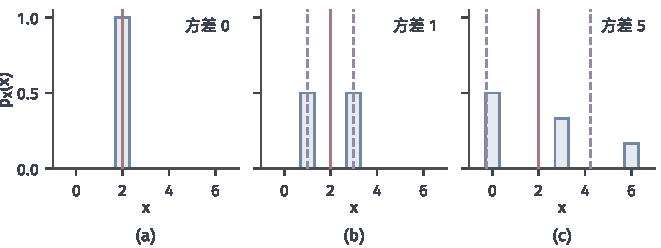
\includegraphics[width=112mm]{figures/07-probability/01-elementary-probability/matplotlib/rvm-same-mean/figure.pdf}
 \caption{三张均值都是$2$的概率表。(a)恒取$2$；(b)以各$\tfrac12$的概率取$1,3$；(c)奖金表。红线是均值，紫色虚线是均值加减标准差$\sqrt{\operatorname{Var}(X)}$。均值相同，方差依次为$0,1,5$。}
 \label{fig:rvm-same-mean}
\end{BookInlineFigure}

力学里也有同样的量。把单位质量按概率放在数轴上，到重心距离的平方乘质量再求和，就是这组质量绕重心的转动惯量。质量离重心越远，转动惯量越大，转动起来越费力。图~\ref{fig:rvm-variance-squares}把奖金表的每个偏差画成正方形，转动惯量就是这些正方形面积的概率加权和。这个类比在一处不完全对应：物理的转动惯量对任何有限质量分布都有限，而概率质量可以分布到无穷远，平方加权和可能是$+\infty$。

\begin{BookInlineFigure}
 \centering
 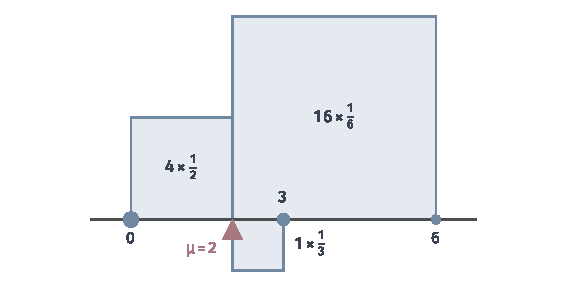
\includegraphics[width=96mm]{figures/07-probability/01-elementary-probability/matplotlib/rvm-variance-squares/figure.pdf}
 \caption{奖金表的方差是偏差平方的加权平均。三个取值到均值$\mu=2$的距离是$2,1,4$，对应正方形的面积是$4,1,16$（为避免重叠，$x=3$的正方形画在数轴下方），蓝点大小表示概率。按概率加权，$4\times\tfrac12+1\times\tfrac13+16\times\tfrac16=5$。}
 \label{fig:rvm-variance-squares}
\end{BookInlineFigure}

\paragraph{方差的定义}
平方的平均有意义，需要先有均值，并且平方的加权和有限。下面的定义把这两项要求都放在“$X^{2}$的期望有限”这一个条件里。

\begin{definition}[方差]
\label{def:rvm-variance}
设$\mathbb{E}[X^{2}]<\infty$，记$\mu=\mathbb{E}[X]$。称
\begin{equation}
 \operatorname{Var}(X)=\mathbb{E}\bigl[(X-\mu)^{2}\bigr]
 \label{eq:rvm-variance}
\end{equation}
为$X$的\term{方差}（variance），也记作$\sigma^{2}$或$\sigma_X^{2}$。
\end{definition}

条件$\mathbb{E}[X^{2}]<\infty$同时保证了均值有限和方差有限。由$(\lvert x\rvert-1)^{2}\geq0$得$\lvert x\rvert\leq\frac12(1+x^{2})$，所以
\[
 \mathbb{E}\lvert X\rvert\leq\tfrac12\bigl(1+\mathbb{E}[X^{2}]\bigr)<\infty .
\]
再由$(x-\mu)^{2}\leq2x^{2}+2\mu^{2}$，又得到
\[
 \mathbb{E}\bigl[(X-\mu)^{2}\bigr]\leq2\,\mathbb{E}[X^{2}]+2\mu^{2}<\infty .
\]这两步都是函数期望的比较，用到了保序性。

均值有限并不保证方差有限。密度$f_X(x)=2x^{-3}$（$x\geq1$）的均值是
\[
 \mathbb{E}[X]=\int_1^{\infty}x\cdot2x^{-3}\,\mathrm{d}x=2,
\]
但
\[
 \mathbb{E}[X^{2}]=\int_1^{\infty}x^{2}\cdot2x^{-3}\,\mathrm{d}x=\int_1^{\infty}\frac{2}{x}\,\mathrm{d}x=+\infty .
\]这时$(X-2)^{2}$是非负变量，它的期望按定义~\ref{def:rvm-expectation}等于$+\infty$，我们说$X$的方差无穷或不是有限的。远处的质量衰减得足以使一次方的力矩有限，却不足以使平方的力矩有限。

图~\ref{fig:rvm-same-mean}中三张表的方差分别是
\[
 0,\qquad (1-2)^{2}\cdot\tfrac12+(3-2)^{2}\cdot\tfrac12=1,\qquad 4\cdot\tfrac12+1\cdot\tfrac13+16\cdot\tfrac16=5 .
\]
方差的大小顺序与图中质量散开的程度一致。

\paragraph{方差为零}
方差是非负变量的期望，所以$\operatorname{Var}(X)\geq0$。方差为零意味着什么？它与“均值是某个数”不是一回事：图~\ref{fig:rvm-same-mean}中三张表的均值都是$2$，只有(a)的方差为零。下面说明方差为零恰好刻画了取值不变的变量。

\begin{theorem}[方差为零的变量]
\label{thm:rvm-zero-variance}
设$\mathbb{E}[X^{2}]<\infty$，$\mu=\mathbb{E}[X]$。
\begin{enumerate}
 \item 若$X$离散，则$\operatorname{Var}(X)=0$当且仅当$\mathbb{P}(X=\mu)=1$。
 \item 若$X$有密度，则$\operatorname{Var}(X)>0$。
\end{enumerate}
\end{theorem}

\begin{proof}
离散情形。$\operatorname{Var}(X)=\sum_i(x_i-\mu)^{2}p_X(x_i)$是非负项之和，它为零当且仅当每个$p_X(x_i)>0$的取值都满足$x_i=\mu$，即全部概率都在$\mu$上。

密度情形。取$\delta>0$，记$A_{\delta}=\{x:\lvert x-\mu\rvert\geq\delta\}$。在$A_{\delta}$上被积函数$(x-\mu)^{2}f_X(x)\geq\delta^{2}f_X(x)$，其余部分非负，所以
\[
 \operatorname{Var}(X)\geq\delta^{2}\int_{A_{\delta}}f_X(x)\,\mathrm{d}x=\delta^{2}\Bigl(1-\int_{\mu-\delta}^{\mu+\delta}f_X(x)\,\mathrm{d}x\Bigr) .
\]
$\delta\to0$时，长度趋于零的区间上的积分趋于零，所以对足够小的$\delta$，括号内大于$\tfrac12$，右边为正。
\end{proof}

这个结论把“数值恒定”说得很准确。方差为零的离散变量以概率一等于均值；若样本空间中还有概率为零的样本点，变量在那里可以取别的值，但这不影响任何概率和期望。有密度的变量把质量铺在一段长度上，不可能全部集中在一点，方差必然为正。对一般的随机变量，同样的刻画在第~\ref{chap:probability-spaces}章证明。

\subsection{计算}
\label{sec:rvm-variance-computation}

按定义计算方差需要两步：先求均值$\mu$，再对$(x-\mu)^{2}$加权求和或积分。对概率表与密度，两个公式分别是
\begin{equation}
 \operatorname{Var}(X)=\sum_{i}(x_i-\mu)^{2}p_X(x_i),\qquad
 \operatorname{Var}(X)=\int_{-\infty}^{\infty}(x-\mu)^{2}f_X(x)\,\mathrm{d}x .
 \label{eq:rvm-variance-formulas}
\end{equation}
它们是函数期望定理~\ref{thm:rvm-lotus}取$g(x)=(x-\mu)^{2}$的特殊情形。对密度$2x$，$\mu=\tfrac23$，展开被积函数后逐项积分，得到
\[
 \operatorname{Var}(X)=\int_0^12x\Bigl(x^{2}-\tfrac43x+\tfrac49\Bigr)\mathrm{d}x
 =2\Bigl(\tfrac14-\tfrac49+\tfrac29\Bigr)=\tfrac{1}{18} .
\]

把展开放在期望外面做，就得到一个通常更方便的公式，它只需要$\mathbb{E}[X]$与$\mathbb{E}[X^{2}]$。

\begin{theorem}[方差的展开式]
\label{thm:rvm-variance-shortcut}
设$\mathbb{E}[X^{2}]<\infty$，则
\begin{equation}
 \operatorname{Var}(X)=\mathbb{E}[X^{2}]-\bigl(\mathbb{E}[X]\bigr)^{2} .
 \label{eq:rvm-variance-shortcut}
\end{equation}
\end{theorem}

\begin{proof}
记$\mu=\mathbb{E}[X]$。$(X-\mu)^{2}=X^{2}-2\mu X+\mu^{2}$，右边三项都可积。由线性性，
\[
 \mathbb{E}\bigl[(X-\mu)^{2}\bigr]=\mathbb{E}[X^{2}]-2\mu\,\mathbb{E}[X]+\mu^{2}=\mathbb{E}[X^{2}]-\mu^{2} .
\]
\end{proof}

用展开式重算两个贯穿例子。奖金表的$\mathbb{E}[X^{2}]=9$，$\mathbb{E}[X]=2$，于是$\operatorname{Var}(X)=9-4=5$。密度$2x$的$\mathbb{E}[X^{2}]=\tfrac12$已在函数期望中算过，于是
\[
 \operatorname{Var}(X)=\tfrac12-\Bigl(\tfrac23\Bigr)^{2}=\tfrac{9-8}{18}=\tfrac{1}{18} .
\]
两个结果都与按定义计算的一致。由于方差非负，式~\eqref{eq:rvm-variance-shortcut}也重新给出了$\mathbb{E}[X^{2}]\geq(\mathbb{E}[X])^{2}$，这是\term{Jensen不等式}在$f(x)=x^{2}$时的情形。

把式~\eqref{eq:rvm-variance-shortcut}与上一节的式~\eqref{eq:rvm-square-error}放在一起，得到对任意常数$c$成立的分解
\begin{equation}
 \mathbb{E}\bigl[(X-c)^{2}\bigr]=\operatorname{Var}(X)+(\mathbb{E}[X]-c)^{2} .
 \label{eq:rvm-parallel-axis}
\end{equation}
用转动惯量的语言，它说绕任一点$c$的转动惯量等于绕重心的转动惯量加上重心到$c$的距离平方，这是力学中的平行轴定理。图~\ref{fig:rvm-error-curves}(a)中抛物线的最低值$5$就是奖金表的方差。

\paragraph{两种算法的比较}
按定义计算时，每一项$(x_i-\mu)^{2}$都非负，结果天然非负，但必须先算出$\mu$再回头处理每个取值；展开式只需要分别累计$x_i$与$x_i^{2}$的加权和，一遍就能完成，求积分时常常也更简单。代价在于展开式是两个可能很大的数相减。

把奖金表的每个取值都加上$10^{8}$，方差仍是$5$。用双精度浮点数计算，$\mathbb{E}[X^{2}]$与$(\mathbb{E}[X])^{2}$都约为$10^{16}$，而这个量级上相邻两个浮点数相差$2$，两数之差只剩下很少的有效数字。实际计算得到$4$；平移量增大到$10^{9}$时，展开式给出$0$。按定义先减去均值再平方，两种平移下得到的都是$5$。所以手算或求解析式时常用展开式，而均值相对波动很大的数值计算应先中心化。

\subsection{平移与缩放}
\label{sec:rvm-variance-affine}

参加一次奖金游戏要付$2$元，净收益是$X-2$；把赌注加倍，奖金变成$2X$；站在庄家一边，收益是$-X$。这些变量的方差与$X$的方差有什么关系？它们都是$aX+b$的形式，答案由中心化后的偏差决定。

\begin{theorem}[方差的平移与缩放]
\label{thm:rvm-variance-affine}
设$\mathbb{E}[X^{2}]<\infty$，$a,b$为实数。则$\mathbb{E}[(aX+b)^{2}]<\infty$，且
\begin{equation}
 \mathbb{E}[aX+b]=a\,\mathbb{E}[X]+b,\qquad \operatorname{Var}(aX+b)=a^{2}\operatorname{Var}(X) .
 \label{eq:rvm-variance-affine}
\end{equation}
\end{theorem}

\begin{proof}
$(ax+b)^{2}\leq2a^{2}x^{2}+2b^{2}$，所以$(aX+b)^{2}$可积。均值的公式是线性性。记$\mu=\mathbb{E}[X]$，新变量的偏差是
\[
 (aX+b)-(a\mu+b)=a(X-\mu),
\]
平移量$b$在相减时消去。平方后取期望，得到
\[
 \operatorname{Var}(aX+b)=\mathbb{E}\bigl[a^{2}(X-\mu)^{2}\bigr]=a^{2}\operatorname{Var}(X) .
\]
\end{proof}

平移整体移动所有取值，不改变它们之间的距离，所以方差不变；缩放把每个偏差乘以$a$，平方后方差乘以$a^{2}$。图~\ref{fig:rvm-shift-scale}画出了奖金表的三个变换：$X-2$的均值是$0$，方差仍是$5$；$2X$的均值是$4$，方差是$4\times5=20$；$-X$把分布左右翻转，均值是$-2$，方差仍是$5$，因为$(-1)^{2}=1$。

\begin{BookInlineFigure}
 \centering
 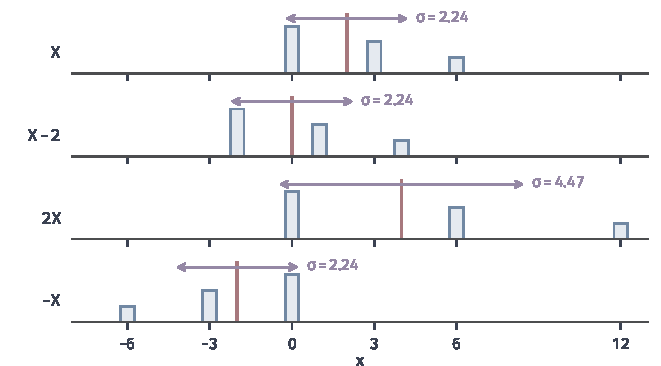
\includegraphics[width=112mm]{figures/07-probability/01-elementary-probability/matplotlib/rvm-shift-scale/figure.pdf}
 \caption{奖金表$X$及其平移、缩放与反射。红线是均值，紫色双箭头是均值加减一个标准差。$X-2$整体左移，宽度不变；$2X$的取值间距加倍，标准差从$2.24$变为$4.47$；$-X$左右翻转，标准差不变。}
 \label{fig:rvm-shift-scale}
\end{BookInlineFigure}

两个特殊情形值得核对。$a=0$时$aX+b$是常数$b$，公式给出方差$0$，与定理~\ref{thm:rvm-zero-variance}一致。$a<0$时缩放同时带来反射，方差只与$\lvert a\rvert$有关，波动的大小不区分方向。

式~\eqref{eq:rvm-variance-affine}只处理一个变量的线性函数。两个不同变量相加时，偏差的平方会产生交叉项。例如$X+X=2X$的方差是$4\operatorname{Var}(X)=20$，而不是$\operatorname{Var}(X)+\operatorname{Var}(X)=10$，多出的$10$正来自交叉项$2\,\mathbb{E}[(X-\mu)(X-\mu)]$。一般的和的方差由协方差描述，在第~\ref{chap:random-vectors}章计算。

\subsection{标准差与标准化}
\label{sec:rvm-standardization}

奖金以元为单位，方差的单位却是“平方元”，$5$平方元很难与$2$元的均值直接比较。开平方就回到原来的单位。

\begin{definition}[标准差]
\label{def:rvm-std}
设$\mathbb{E}[X^{2}]<\infty$。称方差的非负平方根
\begin{equation}
 \sigma_X=\sqrt{\operatorname{Var}(X)}
 \label{eq:rvm-std}
\end{equation}
为$X$的\term{标准差}（standard deviation）。
\end{definition}

奖金表的标准差是$\sqrt5\approx2.24$元，密度$2x$的标准差是$1/\sqrt{18}\approx0.236$。由式~\eqref{eq:rvm-variance-affine}，$\sigma_{aX+b}=\lvert a\rvert\sigma_X$：标准差与变量同步缩放，单位换算时直接乘以换算系数。标准差可以解读为偏差的典型大小，但它是平方平均的平方根，不是平均偏差：奖金表的$\mathbb{E}\lvert X-2\rvert=2$，比$\sqrt5$小，因为平方放大了远处那个偏差$4$的分量。偏离均值超过若干个标准差的概率有多大，要用第~\ref{chap:tail-probabilities}章的尾概率工具估计。

\paragraph{标准化}
均值和标准差分别给出位置和尺度。把它们都除去，就得到一个与单位和位置无关的变量，便于比较不同量纲的随机量，或者描述“偏离均值多少个标准差”。

\begin{definition}[标准化]
\label{def:rvm-standardize}
设$\mathbb{E}[X^{2}]<\infty$且$\sigma_X>0$，$\mu=\mathbb{E}[X]$。称
\begin{equation}
 Z=\frac{X-\mu}{\sigma_X}
 \label{eq:rvm-standardize}
\end{equation}
为$X$的\term{标准化}（standardization）。由式~\eqref{eq:rvm-variance-affine}取$a=1/\sigma_X$，$b=-\mu/\sigma_X$，得$\mathbb{E}[Z]=0$，$\operatorname{Var}(Z)=1$。
\end{definition}

两个条件都不能少。方差必须有限，否则没有可除的尺度；方差必须为正，常数变量没有波动，无法放大成方差为一的变量。

对奖金表，$Z=(X-2)/\sqrt5$以概率$\tfrac12,\tfrac13,\tfrac16$取
\[
 -\tfrac{2}{\sqrt5}\approx-0.89,\qquad \tfrac{1}{\sqrt5}\approx0.45,\qquad \tfrac{4}{\sqrt5}\approx1.79 .
\]
直接核对均值与方差：
\[
 \mathbb{E}[Z]=\tfrac{1}{\sqrt5}\bigl(-1+\tfrac13+\tfrac23\bigr)=0,\qquad
 \mathbb{E}[Z^{2}]=\tfrac15\bigl(2+\tfrac13+\tfrac83\bigr)=1 .
\]对密度$2x$，$Z=\sqrt{18}\,(X-\tfrac23)$的取值范围是$(-2\sqrt2,\sqrt2)$。

\begin{BookInlineFigure}
 \centering
 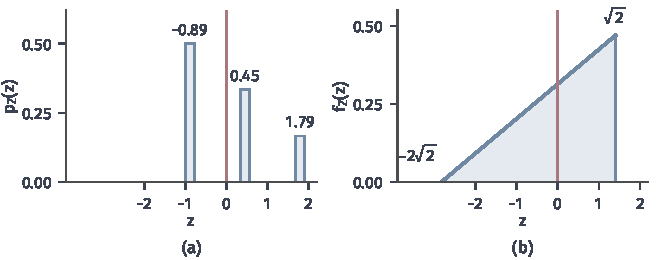
\includegraphics[width=112mm]{figures/07-probability/01-elementary-probability/matplotlib/rvm-standardized/figure.pdf}
 \caption{标准化不改变分布的形状。(a)奖金表标准化后的概率表；(b)密度$2x$标准化后的密度，支撑为$(-2\sqrt2,\sqrt2)$。两者均值都是$0$（红线）、方差都是$1$，但一个是右侧拖尾的三点分布，一个是向右上升的三角形，都不是钟形。}
 \label{fig:rvm-standardized}
\end{BookInlineFigure}

图~\ref{fig:rvm-standardized}说明标准化只做平移和正的缩放，概率表的相对位置和密度的形状都原样保留。均值为零、方差为一并不意味着分布接近某个特定形状，标准化后的奖金仍然只取三个值，仍然向右偏。许多独立小扰动之和标准化后才会接近钟形，那是第~\ref{chap:central-limit-theorem}章的定理，需要独立性和求和，不是标准化本身的效果。


\section{矩}
\label{sec:rvm-moments}

均值是$X$的期望，方差是$(X-\mu)^{2}$的期望。把一次方、二次方换成更高的幂，就得到一族数值特征。奖金表与密度$2x$的均值和方差都已算出，但前者向右拖着一个远处的取值，后者的质量堆在右端，这样的形状差别要靠三次、四次的平均来记录。本节先区分几种矩，再讨论它们何时存在、怎样计算，最后用标准化的三阶和四阶矩描述偏斜与尾部，并说明有限个矩能刻画分布到什么程度。

\subsection{定义}
\label{sec:rvm-moment-definition}

幂次不同，平均对偏差的处理方式也不同。奇数次幂保留偏差的符号，正负偏差会相互抵消；偶数次幂和绝对值的幂不分方向，只记偏差的大小。幂次越高，远处的取值占的权重越大：图~\ref{fig:rvm-power-weights}(a)中$\lvert x\rvert^{p}$在$\lvert x\rvert<1$时随$p$增大而变小，在$\lvert x\rvert>1$时随$p$增大而迅速变大。

\begin{definition}[矩]
\label{def:rvm-moments}
设$k$是正整数，$p>0$是实数。
\begin{enumerate}
 \item 若$\mathbb{E}\lvert X\rvert^{k}<\infty$，称
 \begin{equation}
  m_k=\mathbb{E}[X^{k}]
  \label{eq:rvm-raw-moment}
 \end{equation}
 为$X$的$k$阶\term{原点矩}（raw moment）。
 \item 若$\mathbb{E}\lvert X\rvert^{k}<\infty$，记$\mu=\mathbb{E}[X]$，称
 \begin{equation}
  c_k=\mathbb{E}\bigl[(X-\mu)^{k}\bigr]
  \label{eq:rvm-central-moment}
 \end{equation}
 为$X$的$k$阶\term{中心矩}（central moment）。
 \item 称
 \begin{equation}
  \mathbb{E}\lvert X\rvert^{p}\in[0,+\infty]
  \label{eq:rvm-absolute-moment}
 \end{equation}
 为$X$的$p$阶\term{绝对矩}（absolute moment）；$\mathbb{E}\lvert X-\mu\rvert^{p}$称为$p$阶绝对中心矩。
\end{enumerate}
这些量统称为\term{矩}（moment）。
\end{definition}

在这套记号下，均值是$m_1$，方差是$c_2$，并且$c_1=0$。三类矩的存在条件不同。绝对矩是非负变量的期望，总有意义，只是可能为$+\infty$；阶数$p$可以是任意正实数，例如$\mathbb{E}\lvert X\rvert^{1/2}$。原点矩和中心矩是有符号变量的期望，要求相应的绝对矩有限，阶数取正整数，使$x^{k}$对负数也有定义。中心矩还需要先有均值；下一小节将说明，$\mathbb{E}\lvert X\rvert^{k}<\infty$（$k\geq1$）已经保证了均值有限，也保证了$(X-\mu)^{k}$可积。

\begin{BookInlineFigure}
 \centering
 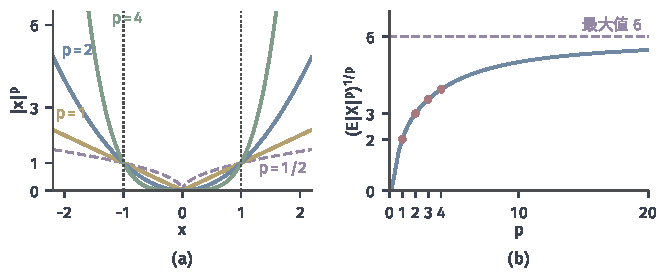
\includegraphics[width=112mm]{figures/07-probability/01-elementary-probability/matplotlib/rvm-power-weights/figure.pdf}
 \caption{幂次与权重。(a)$\lvert x\rvert^{p}$在$p=\tfrac12,1,2,4$时的图像：$\lvert x\rvert<1$时幂次越高权重越小，$\lvert x\rvert>1$时越大，所有曲线在$\lvert x\rvert=1$处（点线）相交。(b)奖金表的$(\mathbb{E}\lvert X\rvert^{p})^{1/p}$随$p$单调增加（蓝），红点是$p=1,2,3,4$时的值$2,3,3.56,3.95$，$p\to\infty$时趋于最大取值$6$（紫色虚线）。}
 \label{fig:rvm-power-weights}
\end{BookInlineFigure}

\paragraph{贯穿例子的矩}
奖金表只取有限个值，各阶矩都存在。由函数期望公式，
\[
 \begin{gathered}
 m_1=2,\qquad m_2=9,\\
 m_3=27\cdot\tfrac13+216\cdot\tfrac16=45,\qquad m_4=81\cdot\tfrac13+1296\cdot\tfrac16=243 .
 \end{gathered}
\]
它的中心矩可以直接从偏差$-2,1,4$计算，例如
\[
 c_3=(-2)^{3}\cdot\tfrac12+1^{3}\cdot\tfrac13+4^{3}\cdot\tfrac16=-4+\tfrac13+\tfrac{32}{3}=7 .
\]
原点矩全为正，因为奖金非负；三阶中心矩为正，是因为偏差$4$的立方$64$远大于偏差$-2$的立方的绝对值$8$，即使后者的概率是前者的三倍。

\subsection{存在性}
\label{sec:rvm-moment-existence}

方差的定义要求$\mathbb{E}[X^{2}]<\infty$，并说明了这一条件蕴含均值有限。同样的道理对一般的阶都成立：高阶矩有限，低阶矩必然有限。

\begin{theorem}[矩的单调存在性]
\label{thm:rvm-moment-monotone}
设$0<p<q$。若$\mathbb{E}\lvert X\rvert^{q}<\infty$，则
\begin{equation}
 \mathbb{E}\lvert X\rvert^{p}\leq1+\mathbb{E}\lvert X\rvert^{q}<\infty .
 \label{eq:rvm-moment-monotone}
\end{equation}
\end{theorem}

\begin{proof}
对每个实数$x$有$\lvert x\rvert^{p}\leq1+\lvert x\rvert^{q}$：若$\lvert x\rvert\leq1$，则$\lvert x\rvert^{p}\leq1$；若$\lvert x\rvert>1$，则$\lvert x\rvert^{p}<\lvert x\rvert^{q}$。把$x$换成$X$并取期望，由保序性即得。
\end{proof}

证明把数轴分成两部分处理。在$\lvert x\rvert\leq1$的近处，所有幂都不超过$1$，总质量又是$1$，所以近处的贡献总是有限的；矩是否存在完全取决于远处，而在远处高次幂压过低次幂。于是$\mathbb{E}\lvert X\rvert^{k}<\infty$蕴含$\mathbb{E}\lvert X\rvert<\infty$，均值存在；再由不等式
\[
 \lvert x-\mu\rvert^{k}\leq2^{k-1}\bigl(\lvert x\rvert^{k}+\lvert\mu\rvert^{k}\bigr),
\]
$(X-\mu)^{k}$也可积，中心矩$c_k$有定义。最后这个不等式来自$t\mapsto t^{k}$在$[0,\infty)$上的凸性。对$a,b\geq0$，凸性给出
\[
 \Bigl(\frac{a+b}{2}\Bigr)^{k}\leq\frac{a^{k}+b^{k}}{2},
\]
再取$a=\lvert x\rvert$，$b=\lvert\mu\rvert$，并利用$\lvert x-\mu\rvert\leq a+b$，两边乘$2^{k}$即得。

\paragraph{定量的比较}
式~\eqref{eq:rvm-moment-monotone}只说明存在，常数$1$也比较粗糙。用Jensen不等式可以得到一个精确的比较：把各阶绝对矩开相应次方，化成同一单位后，它们随阶数单调增加。

\begin{theorem}[Lyapunov不等式]
\label{thm:rvm-lyapunov}
设$0<p<q$且$\mathbb{E}\lvert X\rvert^{q}<\infty$。则
\begin{equation}
 \bigl(\mathbb{E}\lvert X\rvert^{p}\bigr)^{1/p}\leq\bigl(\mathbb{E}\lvert X\rvert^{q}\bigr)^{1/q} .
 \label{eq:rvm-lyapunov}
\end{equation}
\end{theorem}

\begin{proof}
令$r=q/p>1$，$Y=\lvert X\rvert^{p}$。由定理~\ref{thm:rvm-moment-monotone}，$Y$可积，而$\lvert Y\rvert^{r}=\lvert X\rvert^{q}$也可积。函数$f(t)=\lvert t\rvert^{r}$在整个$\mathbb{R}$上是凸函数，由Jensen不等式，
\[
 \bigl(\mathbb{E}[Y]\bigr)^{r}\leq\mathbb{E}\bigl[Y^{r}\bigr],
\]
其中$\mathbb{E}[Y]=\mathbb{E}\lvert X\rvert^{p}$，$\mathbb{E}[Y^{r}]=\mathbb{E}\lvert X\rvert^{q}$。两边开$q$次方，左边成为$(\mathbb{E}\lvert X\rvert^{p})^{1/p}$，即得式~\eqref{eq:rvm-lyapunov}。
\end{proof}

式~\eqref{eq:rvm-lyapunov}称为\term{Lyapunov不等式}（Lyapunov's inequality）。对奖金表，
\[
 \begin{gathered}
 \mathbb{E}\lvert X\rvert=2,\qquad (\mathbb{E}X^{2})^{1/2}=3,\\
 (\mathbb{E}X^{3})^{1/3}=45^{1/3}\approx3.56,\qquad (\mathbb{E}X^{4})^{1/4}=243^{1/4}\approx3.95 .
 \end{gathered}
\]
图~\ref{fig:rvm-power-weights}(b)画出了整条曲线。阶数越高，平均越看重大的取值，最终趋于最大取值$6$：这是因为只保留取值$6$那一项、或把每个取值都放大到$6$，得到
\[
 \tfrac16\cdot6^{p}\leq\mathbb{E}\lvert X\rvert^{p}\leq6^{p},
\]
开$p$次方后左边是$6\cdot6^{-1/p}$，它在$p\to\infty$时趋于$6$。

\paragraph{反方向不成立}
低阶矩有限不能推出高阶矩有限。考虑一族尾部按幂律衰减的密度
\[
 f_X(x)=\alpha x^{-\alpha-1},\qquad x\geq1,
\]
其中$\alpha>0$。它的总质量是$\bigl[-x^{-\alpha}\bigr]_1^{\infty}=1$。对$p>0$，
\[
 \mathbb{E}[X^{p}]=\int_1^{\infty}\alpha x^{p-\alpha-1}\,\mathrm{d}x
 =\begin{cases}\dfrac{\alpha}{\alpha-p}, & p<\alpha,\\ +\infty, & p\geq\alpha .\end{cases}
\]
被积函数是$x$的$p-\alpha-1$次幂，它在无穷远处可积当且仅当指数小于$-1$，即$p<\alpha$。

取$\alpha=3$，均值是$\tfrac32$，$\mathbb{E}[X^{2}]=3$，方差是$3-\tfrac94=\tfrac34$，但三阶矩是$+\infty$。图~\ref{fig:rvm-moment-existence}画出了截断到$[1,M]$的矩：$p=1,2$时分别趋于$\tfrac32$与$3$，$p=3$时等于$3\ln M$，无界增长。取$\alpha=\tfrac32$，均值是$3$而方差无穷；取$\alpha=1$，连均值都是$+\infty$。参数$\alpha$恰好是使矩存在的阶数的上界，它刻画了尾部的厚薄。

\begin{BookInlineFigure}
 \centering
 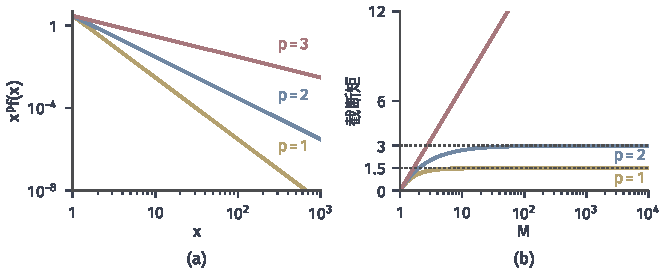
\includegraphics[width=112mm]{figures/07-probability/01-elementary-probability/matplotlib/rvm-moment-existence/figure.pdf}
 \caption{密度$f(x)=3x^{-4}$（$x\geq1$）的矩。(a)双对数坐标下的被积函数$x^{p}f(x)=3x^{p-4}$是直线，斜率为$p-4$；$p=3$时斜率为$-1$，衰减不足以使积分有限。(b)截断矩$\int_1^{M}x^{p}f(x)\,\mathrm{d}x$：$p=1$（黄）与$p=2$（蓝）分别趋于$1.5$与$3$（点线），$p=3$（红）按$3\ln M$增长。}
 \label{fig:rvm-moment-existence}
\end{BookInlineFigure}

离散的例子也一样。第~\ref{sec:rvm-expectation-definition}小节的$p_X(k)=1/[k(k+1)]$满足$k^{p}p_X(k)\leq k^{p-2}$，所以$p<1$时$\mathbb{E}[X^{p}]$有限，而均值是$+\infty$。下表把这些要求的强弱排在一起，每一行的条件蕴含它上面各行的条件。

\begin{BookInlineTable}
 \centering
 \caption{有限矩的要求，以$f(x)=\alpha x^{-\alpha-1}$（$x\geq1$）为例。}
 \label{tab:rvm-moment-requirements}
 \begin{tabular}{lll}
  \toprule
  要求 & 条件 & 使之成立的$\alpha$\\
  \midrule
  均值有限 & $\mathbb{E}\lvert X\rvert<\infty$ & $\alpha>1$\\
  方差有限 & $\mathbb{E}[X^{2}]<\infty$ & $\alpha>2$\\
  偏度有定义 & $\mathbb{E}\lvert X\rvert^{3}<\infty$ & $\alpha>3$\\
  峰度有定义 & $\mathbb{E}[X^{4}]<\infty$ & $\alpha>4$\\
  \bottomrule
 \end{tabular}
\end{BookInlineTable}

\subsection{计算}
\label{sec:rvm-moment-computation}

计算矩就是对幂函数使用函数期望公式，再逐项检查可积性。对密度$2x$，
\[
 m_k=\int_0^1x^{k}\cdot2x\,\mathrm{d}x=\frac{2}{k+2},
\]
于是$m_1=\tfrac23$，$m_2=\tfrac12$，$m_3=\tfrac25$，$m_4=\tfrac13$。直接计算中心矩要展开$(x-\tfrac23)^{k}$再积分，比较繁琐。更好的办法是先算原点矩，再用二项式展开换算。

\begin{theorem}[原点矩与中心矩的换算]
\label{thm:rvm-moment-conversion}
设$k$是正整数，$\mathbb{E}\lvert X\rvert^{k}<\infty$，$\mu=m_1$，并约定$m_0=c_0=1$。则
\begin{align}
 c_k&=\sum_{j=0}^{k}\binom{k}{j}m_j\,(-\mu)^{k-j},
 \label{eq:rvm-central-from-raw}\\
 m_k&=\sum_{j=0}^{k}\binom{k}{j}c_j\,\mu^{k-j}.
 \label{eq:rvm-raw-from-central}
\end{align}
\end{theorem}

\begin{proof}
由定理~\ref{thm:rvm-moment-monotone}，$j\leq k$时$\mathbb{E}\lvert X\rvert^{j}<\infty$，各$m_j$都是有限数。对$(X-\mu)^{k}$用二项式定理，
\[
 (X-\mu)^{k}=\sum_{j=0}^{k}\binom{k}{j}X^{j}(-\mu)^{k-j},
\]
右边是有限个可积变量的线性组合，由线性性逐项取期望得式~\eqref{eq:rvm-central-from-raw}。把$X$写成$(X-\mu)+\mu$再展开，同样得到式~\eqref{eq:rvm-raw-from-central}。
\end{proof}

$k=2$时式~\eqref{eq:rvm-central-from-raw}就是方差展开式$c_2=m_2-\mu^{2}$。$k=3,4$时，代入$m_1=\mu$并合并同类项，得到
\[
 c_3=m_3-3\mu m_2+2\mu^{3},\qquad c_4=m_4-4\mu m_3+6\mu^{2}m_2-3\mu^{4} .
\]

用这两个式子重算奖金表，$\mu=2$。三阶中心矩是
\[
 c_3=45-3\cdot2\cdot9+2\cdot8=7,
\]
与按偏差计算的结果一致。四阶中心矩是
\[
 c_4=243-4\cdot2\cdot45+6\cdot4\cdot9-3\cdot16=243-360+216-48=51 .
\]
对密度$2x$，$\mu=\tfrac23$，代入$m_2=\tfrac12$，$m_3=\tfrac25$，$m_4=\tfrac13$，通分到分母$135$，得到
\[
 c_3=\tfrac25-1+\tfrac{16}{27}=-\tfrac{1}{135},\qquad
 c_4=\tfrac13-\tfrac{16}{15}+\tfrac{4}{3}-\tfrac{16}{27}=\tfrac{1}{135} .
\]
这里$c_4$的四项依次是$m_4$、$4\mu m_3=\tfrac{16}{15}$、$6\mu^{2}m_2=\tfrac43$与$3\mu^{4}=\tfrac{16}{27}$。

\paragraph{平移与缩放}
设$Y=aX+b$。偏差$Y-\mathbb{E}[Y]=a(X-\mu)$与$b$无关，所以中心矩只按缩放变化：
\begin{equation}
 c_k(aX+b)=a^{k}c_k(X),\qquad \mathbb{E}\bigl\lvert Y-\mathbb{E}[Y]\bigr\rvert^{p}=\lvert a\rvert^{p}\,\mathbb{E}\lvert X-\mu\rvert^{p} .
 \label{eq:rvm-central-affine}
\end{equation}
奇数阶中心矩在$a<0$时变号，反映了反射把右侧的偏斜变到左侧。原点矩则随平移改变，$\mathbb{E}[(X+b)^{k}]$按二项式展开是$b$的$k$次多项式。

图~\ref{fig:rvm-raw-central}对奖金表画出了这两种行为。由二项式展开，
\[
 \mathbb{E}[(X+b)^{2}]=9+4b+b^{2},\qquad \mathbb{E}[(X+b)^{3}]=45+27b+6b^{2}+b^{3}
\]
都随$b$变化，而二阶、三阶中心矩始终是$5$与$7$。$b=-\mu=-2$时原点矩与中心矩重合，因为这时$X+b$的均值恰为零。中心矩描述的是质量绕重心的分布，与重心放在数轴何处无关。

\begin{BookInlineFigure}
 \centering
 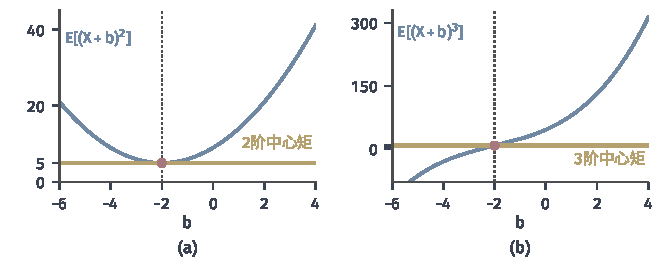
\includegraphics[width=112mm]{figures/07-probability/01-elementary-probability/matplotlib/rvm-raw-central/figure.pdf}
 \caption{平移对原点矩与中心矩的不同影响。对奖金表$X$和平移量$b$：(a)$\mathbb{E}[(X+b)^{2}]$（蓝）是$b$的二次函数，二阶中心矩（黄）恒为$5$；(b)$\mathbb{E}[(X+b)^{3}]$（蓝）是$b$的三次函数，三阶中心矩（黄）恒为$7$。两者在$b=-2$（红点）相交。}
 \label{fig:rvm-raw-central}
\end{BookInlineFigure}

\paragraph{形式展开的陷阱}
换算公式的前提是$\mathbb{E}\lvert X\rvert^{k}<\infty$。缺少这一条时，按形式展开或凭对称性写出的数可能毫无意义。考虑对称的密度
\[
 f_X(x)=\frac{3}{2x^{4}},\qquad \lvert x\rvert\geq1 .
\]
它两侧各有质量$\tfrac12$，均值为$0$，方差是
\[
 \mathbb{E}[X^{2}]=2\int_1^{\infty}x^{2}\cdot\frac{3}{2x^{4}}\,\mathrm{d}x=3\int_1^{\infty}x^{-2}\,\mathrm{d}x=3 .
\]

三阶矩却没有定义：$X^{3}$的正部期望是
\[
 \int_1^{\infty}x^{3}\cdot\frac{3}{2x^{4}}\,\mathrm{d}x=\frac32\int_1^{\infty}\frac{\mathrm{d}x}{x}=+\infty,
\]
负部也是$+\infty$。密度对称会诱使人写下“奇数阶矩为零”，但这只在相应的绝对矩有限时成立，此时被积函数是可积的奇函数。这里$\mathbb{E}\lvert X\rvert^{3}=+\infty$，三阶中心矩和下一小节的偏度都不存在。凡是使用矩的公式，都要先确认它所涉及的最高阶绝对矩有限。

\subsection{偏度与峰度}
\label{sec:rvm-skewness-kurtosis}

三阶中心矩的正负反映偏斜方向，但它的数值带着单位：奖金以元计时$c_3=7$，改用角计时变成$7000$。式~\eqref{eq:rvm-central-affine}说明$c_k$按$a^{k}$缩放，除以$\sigma^{k}$就消去了尺度。等价地，先标准化再求矩。

\begin{definition}[偏度与峰度]
\label{def:rvm-skewness-kurtosis}
设$0<\operatorname{Var}(X)=\sigma^{2}<\infty$，$\mu=\mathbb{E}[X]$，$Z=(X-\mu)/\sigma$。若$\mathbb{E}\lvert X\rvert^{3}<\infty$，称
\begin{equation}
 \gamma_1=\frac{c_3}{\sigma^{3}}=\mathbb{E}[Z^{3}]
 \label{eq:rvm-skewness}
\end{equation}
为$X$的\term{偏度}（skewness）。若$\mathbb{E}[X^{4}]<\infty$，称
\begin{equation}
 \kappa=\frac{c_4}{\sigma^{4}}=\mathbb{E}[Z^{4}]
 \label{eq:rvm-kurtosis}
\end{equation}
为$X$的\term{峰度}（kurtosis），称$\kappa-3$为\term{超额峰度}（excess kurtosis）。
\end{definition}

由式~\eqref{eq:rvm-central-affine}，对$a>0$，$aX+b$与$X$的偏度和峰度都相同；对$a<0$，偏度变号，峰度不变。超额峰度减去的$3$，是下一章将要介绍的高斯分布的峰度。不同文献对“峰度”一词有时指$\kappa$、有时指$\kappa-3$，读数之前要先确认约定。这里讨论的是给定分布的总体量；由观测数据估计偏度和峰度属于统计推断。

两个贯穿例子的值如下。奖金表的
\[
 \gamma_1=\frac{7}{5^{3/2}}\approx0.626,\qquad \kappa=\frac{51}{25}=2.04 .
\]
密度$2x$的方差是$\tfrac{1}{18}$，$\sigma^{3}=1/(54\sqrt2)$，$\sigma^{4}=\tfrac{1}{324}$，于是
\[
 \gamma_1=-\frac{54\sqrt2}{135}=-\frac{2\sqrt2}{5}\approx-0.566,\qquad \kappa=\frac{324}{135}=\frac{12}{5} .
\]
奖金表的偏度为正：远处那个$6$元在均值右侧，立方把它的影响放大。密度$2x$的质量堆在右端，左侧有一条渐渐变薄的长边，偏度为负。

\paragraph{零偏度不保证对称}
若$X$关于$\mu$对称且$\mathbb{E}\lvert X\rvert^{3}<\infty$，则$(X-\mu)^{3}$与$-(X-\mu)^{3}$同分布，$c_3=-c_3$，偏度为零。反过来不成立。设$Y$以概率$\tfrac16,\tfrac12,\tfrac13$取$-5,-1,4$。它的均值和三阶矩分别是
\[
 \mathbb{E}[Y]=-\tfrac56-\tfrac12+\tfrac43=0,\qquad
 \mathbb{E}[Y^{3}]=-\tfrac{125}{6}-\tfrac12+\tfrac{64}{3}=0 .
\]
所以$c_3=0$，偏度为零。但$Y$不对称：取负值的概率是$\tfrac23$，中位数是$-1$而不是均值$0$。图~\ref{fig:rvm-zero-skew}显示，零偏度只是左侧一个远偏差的立方与右侧一个中等偏差的立方恰好抵消。

\begin{BookInlineFigure}
 \centering
 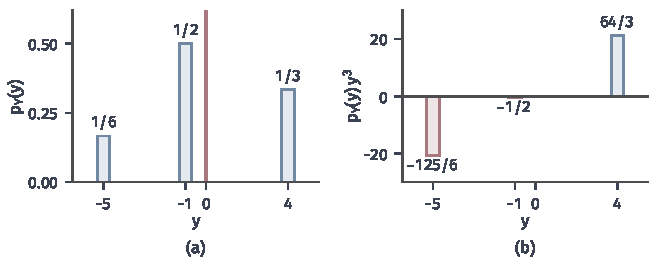
\includegraphics[width=112mm]{figures/07-probability/01-elementary-probability/matplotlib/rvm-zero-skew/figure.pdf}
 \caption{偏度为零的不对称分布。(a)$Y$以概率$\tfrac16,\tfrac12,\tfrac13$取$-5,-1,4$，均值为$0$（红线），方差为$10$。(b)三阶矩的各项贡献$p_Y(y)\,y^{3}$：左侧两项（红）之和$-\tfrac{64}{3}$与右侧一项（蓝）$\tfrac{64}{3}$相互抵消。}
 \label{fig:rvm-zero-skew}
\end{BookInlineFigure}

\paragraph{峰度衡量什么}
由标准化变量$Z$的$\mathbb{E}[Z^{2}]=1$，可以把峰度改写成
\[
 \kappa-1=\mathbb{E}[Z^{4}]-\bigl(\mathbb{E}[Z^{2}]\bigr)^{2}=\operatorname{Var}(Z^{2}) .
\]
这给出了峰度的一个准确读法：它衡量$Z^{2}$在其均值$1$周围的波动。若质量都集中在$\lvert Z\rvert=1$附近，$Z^{2}$几乎不变，峰度接近$1$；若一部分质量在中心附近、另一部分在很远处，$Z^{2}$变化剧烈，峰度就大。所以峰度同时受中心附近和远处的影响，不能只理解为峰的尖锐程度。由这个读法还可以得到峰度与偏度之间的约束。

\begin{theorem}[偏度与峰度的约束]
\label{thm:rvm-pearson}
设$\mathbb{E}[X^{4}]<\infty$且$\operatorname{Var}(X)>0$。则
\begin{equation}
 \kappa\geq1+\gamma_1^{2} .
 \label{eq:rvm-pearson}
\end{equation}
对离散的$X$，等号成立当且仅当$X$以概率一只取两个值。
\end{theorem}

\begin{proof}
记$Z$为标准化变量，考虑非负变量$W=(Z^{2}-\gamma_1Z-1)^{2}$。展开后各项都是$Z$的不超过四次的幂，都可积：
\[
 W=Z^{4}-2\gamma_1Z^{3}+(\gamma_1^{2}-2)Z^{2}+2\gamma_1Z+1 .
\]
代入$\mathbb{E}[Z]=0$，$\mathbb{E}[Z^{2}]=1$，$\mathbb{E}[Z^{3}]=\gamma_1$，$\mathbb{E}[Z^{4}]=\kappa$，由线性性得
\[
 0\leq\mathbb{E}[W]=\kappa-2\gamma_1^{2}+\gamma_1^{2}-2+1=\kappa-\gamma_1^{2}-1 .
\]

等号成立当且仅当$\mathbb{E}[W]=0$。对离散的$X$，这等价于$Z$的每个正概率取值都是二次方程$z^{2}-\gamma_1z-1=0$的根。这个方程的判别式$\gamma_1^{2}+4>0$，恰有两个实根，所以$Z$至多取两个值；它的方差为一，不是常数，因此恰好取两个值。反过来，设$Z$只取两个值$z_1<z_2$，概率分别为$1-r$与$r$。由$\mathbb{E}[Z]=0$得$(1-r)z_1=-rz_2$，代入$\mathbb{E}[Z^{2}]=1$，
\[
 1=(1-r)z_1\cdot z_1+rz_2\cdot z_2=-rz_2z_1-(1-r)z_1z_2=-z_1z_2 .
\]
所以$z_1,z_2$是二次方程$z^{2}-(z_1+z_2)z-1=0$的两个根，于是
\[
 z_k^{2}=(z_1+z_2)z_k+1,\qquad k=1,2 .
\]两边乘$z_k$后取期望，得到
\[
 \gamma_1=\mathbb{E}[Z^{3}]=(z_1+z_2)\,\mathbb{E}[Z^{2}]+\mathbb{E}[Z]=z_1+z_2 .
\]于是$Z$的两个取值都满足$z^{2}-\gamma_1z-1=0$，$W$恒为零，等号成立。
\end{proof}

图~\ref{fig:rvm-skew-kurt-plane}把本节的例子放到偏度—峰度平面上。抛物线$\kappa=1+\gamma_1^{2}$下方的区域不可能出现；两点分布恰好落在抛物线上，例如以概率$\tfrac56,\tfrac16$取$1,7$的表，偏度$4/\sqrt5\approx1.79$，峰度$4.2$。三点或更多点的分布与有密度的分布都在抛物线上方。

\begin{BookInlineFigure}
 \centering
 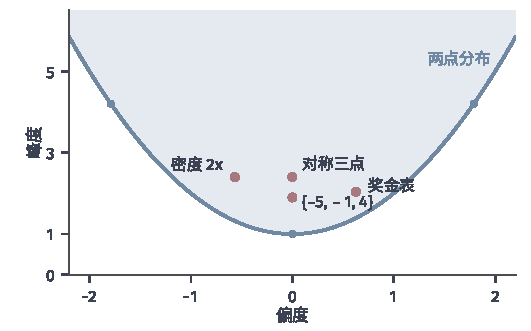
\includegraphics[width=90mm]{figures/07-probability/01-elementary-probability/matplotlib/rvm-skew-kurt-plane/figure.pdf}
 \caption{偏度—峰度平面。可能出现的点位于抛物线$\kappa=1+\gamma_1^{2}$上或其上方（浅蓝区域），两点分布落在抛物线上（蓝点为取值概率$\tfrac16,\tfrac12,\tfrac56$的三例）。红点是本节的例子：奖金表$(0.63,2.04)$，密度$2x$为$(-0.57,2.4)$，$Y$在$\{-5,-1,4\}$上为$(0,1.9)$，对称三点分布为$(0,2.4)$。}
 \label{fig:rvm-skew-kurt-plane}
\end{BookInlineFigure}

\paragraph{峰度不能单独确定形状}
同一个峰度可以对应形状完全不同的分布。设$Z$以概率$q,1-2q,q$取$-a,0,a$。方差为一要求$2qa^{2}=1$，而$\mathbb{E}[Z^{4}]=2qa^{4}=\frac{1}{2q}$。取$q=\tfrac{5}{24}$，峰度是$\tfrac{12}{5}$，与密度$2x$的峰度相同。

图~\ref{fig:rvm-same-kurtosis}把两者并列：一个是向右上升、支撑有界、偏度为负的三角形密度，另一个是对称的三点分布，中间有一个高的质量。两者峰度都是$2.4$，低于$3$。峰度既不能说明峰的尖锐，也不能说明尾部是否有界，它只是$Z^{2}$的波动这一个数。描述尾部的衰减规律要直接看尾概率，第~\ref{chap:tail-probabilities}章会用矩来估计它。

\begin{BookInlineFigure}
 \centering
 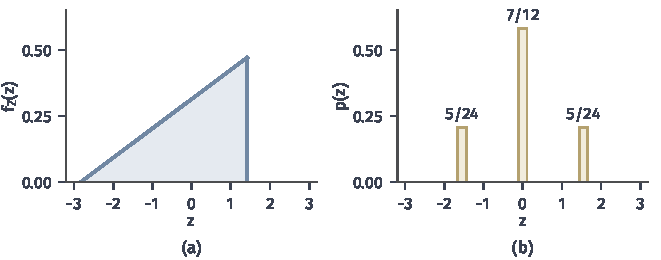
\includegraphics[width=112mm]{figures/07-probability/01-elementary-probability/matplotlib/rvm-same-kurtosis/figure.pdf}
 \caption{峰度相同而形状不同的两个标准化分布。(a)密度$2x$标准化后的三角形密度（蓝），偏度$-0.57$；(b)以概率$\tfrac{5}{24},\tfrac{7}{12},\tfrac{5}{24}$取$-1.55,0,1.55$的对称三点分布（黄），偏度$0$。两者均值为$0$、方差为$1$，峰度都是$12/5$。}
 \label{fig:rvm-same-kurtosis}
\end{BookInlineFigure}

\subsection{矩对分布的刻画}
\label{sec:rvm-moments-characterize}

均值、方差、偏度、峰度一个比一个记录更细的信息。自然要问：知道前几个矩，能否确定分布？如果能，概率表与密度就可以用一串数代替。答案是否定的，而且相差得很远。

\paragraph{均值与方差相同的三张表}
奖金表的均值是$2$，方差是$5$。两点分布的方差有一个简单公式：以概率$1-r$与$r$取$a<b$时，均值$\mu$满足$(1-r)(a-\mu)+r(b-\mu)=0$，方差等于$(b-\mu)(\mu-a)$。要求$\mu=2$、方差为$5$，可取$a=1,b=7$，此时$r=\tfrac16$；也可取$a=-3,b=3$，此时$r=\tfrac56$。

于是三张表以概率$\tfrac12,\tfrac13,\tfrac16$取$0,3,6$，以概率$\tfrac56,\tfrac16$取$1,7$，以概率$\tfrac16,\tfrac56$取$-3,3$，它们的均值都是$2$、方差都是$5$。图~\ref{fig:rvm-same-mean-var}显示它们的形状截然不同：第二张右偏，第三张左偏，偏度分别为$\pm4/\sqrt5\approx\pm1.79$，奖金表的偏度是$0.63$。均值和方差只确定了重心与转动惯量，质量怎样具体分配，它们管不到。

\begin{BookInlineFigure}
 \centering
 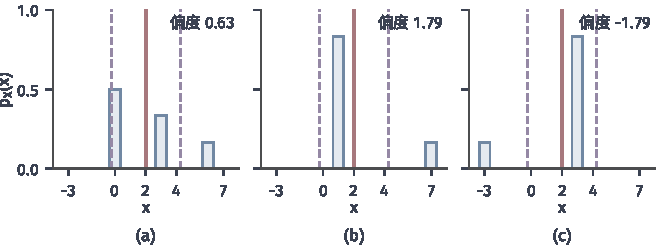
\includegraphics[width=112mm]{figures/07-probability/01-elementary-probability/matplotlib/rvm-same-mean-var/figure.pdf}
 \caption{均值都是$2$（红线）、方差都是$5$的三张概率表，紫色虚线是均值加减标准差$\sqrt5$。(a)奖金表；(b)以概率$\tfrac56,\tfrac16$取$1,7$；(c)以概率$\tfrac16,\tfrac56$取$-3,3$。三者的偏度分别为$0.63$、$1.79$与$-1.79$。}
 \label{fig:rvm-same-mean-var}
\end{BookInlineFigure}

\paragraph{有限个矩不能确定分布}
增加矩的个数也无济于事。只要多给出几个矩，就能用更细的扰动保持它们不变，下面的定理把这一点做成构造。

\begin{theorem}[有限个矩不确定分布]
\label{thm:rvm-finite-moments}
对每个正整数$k$，存在$(0,1)$上的密度$f\neq1$，使以$f$为密度的变量与以常数$1$为密度的变量具有相同的$1,\dots,k$阶矩，而$k+1$阶矩不同。
\end{theorem}

\begin{proof}
寻找次数不超过$k+1$的多项式$q(x)=\sum_{l=0}^{k+1}a_lx^{l}$，使
\begin{equation}
 \int_0^1x^{j}q(x)\,\mathrm{d}x=0,\qquad j=0,1,\dots,k .
 \label{eq:rvm-orthogonal}
\end{equation}
这是关于$k+2$个系数$a_0,\dots,a_{k+1}$的$k+1$个齐次线性方程，未知数多于方程，所以有非零解。非零多项式在$[0,1]$上不恒为零，记$M=\max_{[0,1]}\lvert q\rvert>0$，把$q$换成$q/M$，就可设$\max_{[0,1]}\lvert q\rvert=1$。

令$f=1+q$。它在$(0,1)$上非负，由式~\eqref{eq:rvm-orthogonal}中$j=0$的方程，总积分为一，所以是密度；它不恒等于$1$。对$1\leq j\leq k$，
\[
 \int_0^1x^{j}f(x)\,\mathrm{d}x=\int_0^1x^{j}\,\mathrm{d}x+\int_0^1x^{j}q(x)\,\mathrm{d}x=\int_0^1x^{j}\,\mathrm{d}x,
\]
前$k$阶矩相同。若$k+1$阶矩也相同，则$q$与$1,x,\dots,x^{k+1}$的乘积积分都为零，从而与自身的乘积积分$\int_0^1q^{2}\,\mathrm{d}x=0$，这对非零多项式不可能。
\end{proof}

$k=2$时可以取$q(x)=20x^{3}-30x^{2}+12x-1$。逐项积分可以核对式~\eqref{eq:rvm-orthogonal}：
\[
 \begin{aligned}
 \int_0^1q(x)\,\mathrm{d}x&=5-10+6-1=0,\\
 \int_0^1xq(x)\,\mathrm{d}x&=4-\tfrac{15}{2}+4-\tfrac12=0,\\
 \int_0^1x^{2}q(x)\,\mathrm{d}x&=\tfrac{10}{3}-6+3-\tfrac13=0 .
 \end{aligned}
\]
它在$[0,1]$上的最大绝对值是$1$，在两个端点取到。于是$f=1+q$与常数密度有相同的均值$\tfrac12$和方差$\tfrac1{12}$，三阶矩则多出$\int_0^1x^{3}q\,\mathrm{d}x=\tfrac{1}{140}$。$k=4$时类似地取一个五次多项式。图~\ref{fig:rvm-same-moments}显示，保持的矩越多，扰动的波动越多，但两个密度始终明显不同。

\begin{BookInlineFigure}
 \centering
 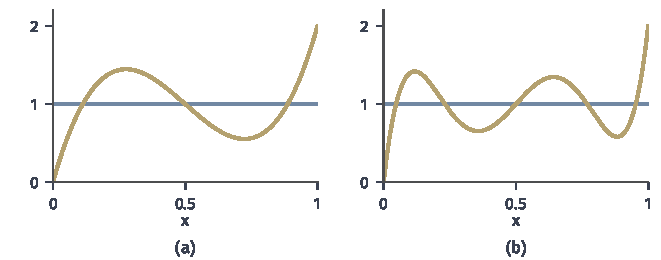
\includegraphics[width=112mm]{figures/07-probability/01-elementary-probability/matplotlib/rvm-same-moments/figure.pdf}
 \caption{前几个矩相同的不同密度。(a)常数密度$1$（蓝）与$1+q(x)$（黄），$q(x)=20x^{3}-30x^{2}+12x-1$，两者的前两阶矩相同；(b)常数密度与$1+252x^{5}-630x^{4}+560x^{3}-210x^{2}+30x-1$，前四阶矩相同。保持的矩越多，扰动振荡越快。}
 \label{fig:rvm-same-moments}
\end{BookInlineFigure}

那么全部矩能否确定分布？结论取决于尾部的轻重。取值有界时，全部矩确实决定分布，证明要用多项式在有界区间上一致逼近连续函数。尾部较重时则不然：存在各阶矩都有限且全部相同的两个不同分布，构造它们要用到第~\ref{chap:random-variable-transformations}章的密度换元，相关讨论可查阅~\scite{math-kallenberg2021probability}。用变换判断两个分布是否相同的系统工具在第~\ref{chap:weak-convergence-of-distributions}章介绍。在那之前，矩应当被看作分布的数值概括：它们回答特定的问题，例如平均、波动、偏斜，但不能代替概率表、分布函数或密度。


\section{本章小结}
\label{sec:rvm-summary}

本章从一张概率表出发，问怎样用少数几个数概括它。期望是概率质量的重心，按概率加权平均取值；方差是绕重心的转动惯量，按概率加权平均偏差的平方；更高阶的矩加重远处偏差的权重，标准化后的三阶、四阶矩描述偏斜方向与$Z^{2}$的波动。奖金表与密度$2x$贯穿全章，表~\ref{tab:rvm-summary}汇总了它们的各项数值。

\begin{BookInlineTable}
 \centering
 \caption{两个贯穿例子的数值特征。}
 \label{tab:rvm-summary}
 \begin{tabular}{lcc}
  \toprule
  数值特征 & 奖金表 & 密度$2x$\\
  \midrule
  均值$\mu$ & $2$ & $2/3$\\
  方差$\sigma^{2}$ & $5$ & $1/18$\\
  标准差$\sigma$ & $2.24$ & $0.236$\\
  三阶中心矩$c_3$ & $7$ & $-1/135$\\
  四阶中心矩$c_4$ & $51$ & $1/135$\\
  偏度$\gamma_1$ & $0.626$ & $-0.566$\\
  峰度$\kappa$ & $2.04$ & $2.4$\\
  \bottomrule
 \end{tabular}
\end{BookInlineTable}

每个数回答一个特定的问题，也需要特定的条件，表~\ref{tab:rvm-summary-roles}把它们与第~\ref{chap:random-variables}章的分位数放在一起比较。均值与中位数都描述位置，前者使平方误差最小、受远处取值牵动，后者使绝对误差最小、只看左右质量的分配。方差与标准差描述波动尺度，标准差与变量同单位。偏度与峰度不随单位改变，却只是两个数，零偏度不保证对称，峰度也不能确定峰形或尾部规律。

\begin{BookInlineTable}
 \centering
 \caption{各数值特征回答的问题、存在条件与在$aX+b$（$a\neq0$）下的变化。偏度与峰度还要求$\sigma>0$。}
 \label{tab:rvm-summary-roles}
 \begin{tabular}{llll}
  \toprule
  特征 & 回答的问题 & 存在条件 & 在$aX+b$下\\
  \midrule
  均值 & 重心在哪里 & $\mathbb{E}\lvert X\rvert<\infty$ & $a\mu+b$\\
  中位数 & 左右各半的位置 & 总存在 & 随之变换\\
  方差 & 绕重心散开多少 & $\mathbb{E}[X^{2}]<\infty$ & $a^{2}\sigma^{2}$\\
  标准差 & 同单位的波动 & $\mathbb{E}[X^{2}]<\infty$ & $\lvert a\rvert\sigma$\\
  $k$阶中心矩 & 偏差的$k$次平均 & $\mathbb{E}\lvert X\rvert^{k}<\infty$ & $a^{k}c_k$\\
  偏度 & 偏斜方向 & $\mathbb{E}\lvert X\rvert^{3}<\infty$ & $a<0$时变号\\
  峰度 & $Z^{2}$的波动 & $\mathbb{E}[X^{4}]<\infty$ & 不变\\
  \bottomrule
 \end{tabular}
\end{BookInlineTable}

存在条件是使用这些数的前提。非负变量的期望总有意义但可能为$+\infty$；有符号变量要分别检查正部与负部，两者都无穷时期望不存在，对称也不能补救。高阶绝对矩有限蕴含低阶绝对矩有限，Lyapunov不等式给出了定量的比较；反方向不成立，幂律尾部的密度$\alpha x^{-\alpha-1}$只有低于$\alpha$阶的矩。一切展开公式和对称性论证都要先确认所涉最高阶的绝对矩有限。

运算规则同样有边界。期望的线性性对可积变量的有限线性组合成立，不需要独立性，信封问题说明它能绕开复杂的依赖结构。乘积的期望一般不能拆开，无穷求和与取期望的交换需要额外条件。函数的期望可以直接用原变量的分布计算，不必求出新变量的分布，但要对每个函数检查绝对可积。凸函数满足Jensen不等式，变量越分散，“先平均再变换”与“先变换再平均”相差越大。方差的展开式便于手算，数值计算中则应先减去均值。

数值特征是分布的概括，不是替代。均值和方差相同的概率表形状可以完全不同；对任意给定的$k$，都有前$k$阶矩相同的不同密度。尾概率的估计、和的方差以及用变换识别分布，分别在第~\ref{chap:tail-probabilities}章、第~\ref{chap:random-vectors}章与第~\ref{chap:weak-convergence-of-distributions}章展开。下一章把本章的工具用于常见分布，在每个模型的试验机制和参数下计算均值与方差，并检查它们是否存在。

